\documentclass[english]{aiaa-tc}
\usepackage{lmodern}
\renewcommand{\sfdefault}{lmss}
\renewcommand{\ttdefault}{lmtt}
\usepackage[T1]{fontenc}
\usepackage[latin9]{inputenc}
\usepackage{array}
\usepackage{multirow}
\usepackage{amssymb}
\usepackage{graphicx}
%\usepackage{nomencl}
% the following is useful when we have the old nomencl.sty package
%\providecommand{\printnomenclature}{\printglossary}
%\providecommand{\makenomenclature}{\makeglossary}
%\makenomenclature
\makeatletter

%%%%%%%%%%%%%%%%%%%%%%%%%%%%%% LyX specific LaTeX commands.
%% Because html converters don't know tabularnewline
\providecommand{\tabularnewline}{\\}
%% A simple dot to overcome graphicx limitations
\newcommand{\lyxdot}{.}


%%%%%%%%%%%%%%%%%%%%%%%%%%%%%% User specified LaTeX commands.
\usepackage{wrapfig}% embedding figures/tables in text (i.e., Galileo style)
 \usepackage{threeparttable}% tables with footnotes
 \usepackage{dcolumn}% decimal-aligned tabular math columns
  \newcolumntype{d}{D{.}{.}{-1}}
 %\usepackage{nomencl}% automatic nomenclature generation via makeindex
  \makeglossary
 \usepackage{subfig}% subcaptions for subfigures
 \usepackage{fancyvrb}% extended verbatim environments
  \fvset{fontsize=\footnotesize,xleftmargin=2em}
 \usepackage{lettrine}% dropped capital at beginning of paragraph
% \usepackage[dvips]{dropping}% alternative dropped capital package
% \usepackage{hyperref}% embedding hyperlinks 
% \usepackage{morefloats}
 % define some commands to maintain consistency
 \newcommand{\pkg}[1]{\texttt{#1}}
 \newcommand{\cls}[1]{\textsf{#1}}
 \newcommand{\file}[1]{\texttt{#1}}

\@ifundefined{showcaptionsetup}{}{%
 \PassOptionsToPackage{caption=false}{subfig}}
\usepackage{subfig}
\makeatother

\usepackage{babel}
\begin{document}
\title{A Study of the Noise Source Mechanisms in an Excited Mach 0.9 Jet - Complementary Experimental and Computational Analysis}


\author{Michael Crawley\thanks{Graduate Research Assistant. Student Member, AIAA}, \
Rachelle L. Speth\thanks{Graduate Research Assistant. Student Member, AIAA},
 Datta V. Gaitonde\thanks{John Glenn Chair Professor. Fellow, AIAA},
 and Mo Samimy\thanks{John B. Nordholt Professor. Fellow, AIAA}
\\\normalsize\itshape Mechanical and Aerospace Engineering, The Ohio State University, Columbus, OH \\}


\maketitle

\begin{abstract}
	Experimental and Numerical databases are used in conjunction with each other to explore the dynamics of large scale structure evolution and the resultant effect on the near and far fields. 
A Mach 0.9 jet excited by plasma actuators to produce consistent coherent structures was studied using correlations. 
The near field was further analyzed using acoustic and hydrodynamic decompositions.
WHAT DID WE FIND?
\end{abstract}

\section{Introduction}
Engine exhaust constitutes one of the major components of aircraft noise during takeoff and landing, and hence poses a significant health concern for community and military personnel. Mitigation of the aeroacoustic noise generated by free jets is therefore a necessity for the both the commercial and military aviation industries. Current noise reduction technologies such as increased bypass ratios or geometric modifications to the nozzle (tabs, chevrons, and lobed mixers), though effective, have associated performance penalties in terms of added weight, drag, or loss of thrust - penalties that are incurred over the entire duration of the flight. A shift to active control technology thus desirable in order to minimize the performance penalties while maximizing the noise reduction, however the proper application of control is not readily apparent. In the simulated two-dimensional shear layer of Wei \& Freund \cite{Wei2006} a generalized actuator was able to reduce the noise along a prescribed line in the acoustic field by up to 11 dB. The researchers observed that the excitation was not altering the broad characteristics of the shear layer (such as turbulent kinetic energy) or even the evolution of the most energetic structures in an appreciable manner. Rather, the control appeared to be effecting the acoustic field by regularizing the large-scale structures, thereby reducing the radiating efficiency of the noise sources. Clearly, fundamental understanding of the noise sources and radiating mechanisms is required for efficient and effective active noise mitigation strategies.

Perhaps the most well-known source model for jet mixing noise is the two-component model of Tam \textit{et al.} \cite{Tam1996}, which recognized that the acoustic far-field spectra of jets can be represented as two distinct universal similarity spectra, irrespective of jet Mach number or temperature ratio. In this model, the incoherent fine-scale mixing layer turbulence, produces an incoherent, broadband acoustic field and is believed to be the dominant source of acoustic radiation at sideline angles. In contrast, aft angle radiation is dominated by the large-scale structures and exhibit a strong spectral peak. Theoretical analysis by Tam \cite{Tam1971} demonstrated Mach wave radiation emitted through the supersonic convective of these large scale structures - the oft-mentioned "wavy-wall" analogy. This analysis was extended in Tam \& Burton \cite{Tam1984} to include amplification and decay of the structures, through which subsonically-convecting structures were found to emit noise (this structure evolution was also shown to broaden the directivity and frequency bands of the acoustic radiation). Experiments utilizing direct correlations between density and velocity fluctuations in the shear layers of high-speed jets and the
acoustic far-field have supported this two-component source model \cite{Panda2002,Panda2005b}.

That the large-scale structures are the dominant noise sources in the turbulent jet is beyond doubt at this point. Yet, the exact dynamics that govern the evolution of the structures and ultimately the noise emission are still not fully understood. The intermittent nature of the structures and noise emission was first observed by Hileman \textit{et al.} \cite{hj2005-1} in a supersonic jet. Simplified source models utilizing temporally and spatially modulated wavepackets were found to reproduce the superdirective character observed in the far-field spectra, as well as improve the match between the observed and predicted spectral amplitudes \cite{Sandham2006,Cavalieri2010,Crighton1990}. Hence, understanding the exact spatiotemporal evolution of the large-scale structures is important to predicting and ultimately controlling their radiation production. 

The ability to perturb the jet shear layer, in effect controlling the temporal and azimuthal frequency content of the large-scale structures, may thus serve as a useful tool for noise source analysis. Localized arc-filament plasma actuators (LAFPAs) have been developed at the Gas Dynamics and Turbulence Laboratory for use in high-speed flow control applications. Unlike traditional acoustic drivers, LAFPAs have been shown to produce high amplitude and high frequency excitation signals suitable for controlling the shear layer development of high Mach number and high Reynolds number jets \cite{sm2004-1,uyg2007-2,sm2007-2,sm2007-3}.These actuators have successfully been used for both mixing enhancement and noise mitigation in laboratory scale subsonic and supersonic jets; a review of the the development of LAFPAs and their use in high-speed jet flow control can be found in Samimy \textit{et al}. \cite{Samimy2012} Additional to their noise mitigation and mixing enhancement potential, LAFPAs have been used as diagnostic tools for understanding the large-scale structure dynamics and noise production mechanisms in high-speed jets. Kearney-Fischer \textit{et al.} \cite{Kearney-Fischer2011a} utilized a phase-locked schlieren imaging system to LAFPA excitation in a heated, subsonic jet in order to study the Mach-wave-like compression waves generated by the large-scale structures. By varying the frequency and Fourier mode of the forcing, the effect of structure coherency on the radiated noise was evaluated. Sinha \textit{et al.} \cite{sinha2013} investigated the dynamics of large-scale structure interactions in a Mach 0.9 jet by phase-averaging the near-field pressure signals from a linear microphone array. It was found that for low to moderate forcing Strouhal numbers ($St_{DF}  <  0.5$), each excitation pulse produced a single structure, the near-field signature of which was a compact waveform. The waveform shape and amplitude at moderate forcing Strouhal numbers were found to be well-predicted by a linear superposition of the impulse response of the jet to excitation ($St_{DF}  <  0.1$). This analysis was extended to the acoustic near- and far-field in Crawley \textit{et al.} \cite{Crawley2015}, in which it was found that the acoustic field could also be represented as a linear superposition of the impulse response of the jet, and that the dominant noise source region shifted upstream with increasing Strouhal number.

Concurrent to this work, the High Fidelity Computational Multi-Physics Laboratory (HFCMPL) has developed a large eddy simulation solver (FDL3DI) to simulate the effect of the LAFPAs on the jet shear layer. Validation of the numerical method and initial comparisons of the simulated and experimental database were performed in Gaitonde \& Samimy \cite{gdv2011-POF} and Speth and Gaitonde \cite{speth2014}. In the recent studies of Speth and Gaitonde \cite{spethASME2013,speth2014}, the LAFPAs were pulsed at low frequencies to analyze the impulse response and at higher frequencies ($St_{DF}>0.15$) to study the manner in which the structures begin to interact. The large coherent structures of the jet were linked to the near field through analysis of phase-averaged waveforms and correlations. The correlations described the development and interaction of subsequent structures in time and space. The higher frequency of excitation tested ($St_{DF}=0.25$) created a narrower correlated region than the low frequency cases due to the organized development and decay of the large scale structures. This region extended from the end of the potential core to the 30 degree near field. Compressibility effects were also investigated in Speth \& Gaitonde \cite{speth2014} and found that the supersonic case has higher correlations throughout the near field than the subsonic cases. 

The current work represents the first stage in assimilating analyses from the experimentally- and numerically-acquired databases to use the strengths of both techniques (i.e. long time traces for experiments and spatial resolution for simulations) to obtain a deeper knowledge of noise production of a jet. First, we begin by describing the experimental and computational setup in Sections \ref{expersetup} and \ref{theo}. Then the evolution of the large scale coherent structures is analyzed in Section \ref{structure}, while the acoustic component of the near field is analyzed in Section \ref{acoustic}.
%Expand this section once we figure out what the hell we are doing....

\section{Experimental Setup\label{expersetup}}
Experimentation was conducted in the free jet facility (a schematic of which can be found in Fig. \ref{GDTLschematic}) at the GDTL within the Ohio State University's Aerospace Research Center.The dimensions of the chamber are 5.14 m wide by 4.48 m long and 2.53 m high (wedge-tip to wedge-tip). The design of the chamber produces an anechoic cutoff frequency of 160 Hz, below the frequencies of interest for this study. Additional details of the facility design and validation can be found in Hahn \cite{Hahn2011}. Compressed, dried, and filtered air is supplied by two cylindrical storage tanks with a total capacity of 43 m$^3$ and maximum pressure of 16 MPa; the tanks are charged by three, five-stage reciprocating compressors. The air enters the facility horizontally, passes through a stagnation chamber and turbulence screens, and exhausts through a converging nozzle. Opposite the nozzle, a collector accumulates the jet and entrained air and exhausts to the outdoors.

A converging, axisymmetric nozzle with exit diameter of 25.4 mm was used in the current study. The internal contour of the nozzle was designed using a fifth order polynomial. The nozzle utilized a thick-lipped design in order to simplify the mounts for the LAFPA extension, which housed the eight actuators used in this study.For the experiments reported in this paper, the jet was operated at a Mach number, $M_{j}$, of 0.90, and with a total temperature ratio of unity.The Reynolds number based on the jet exit diameter was $6.2 \times 10^{5}$; previous investigations using hot-wire anemometry have indicated that the initial shear layer is turbulent for this operating condition with momentum thickness ~0.09 mm and boundary layer thickness ~1 mm \cite{kfm2009-1}. 
\begin{figure}
	\begin{center}
		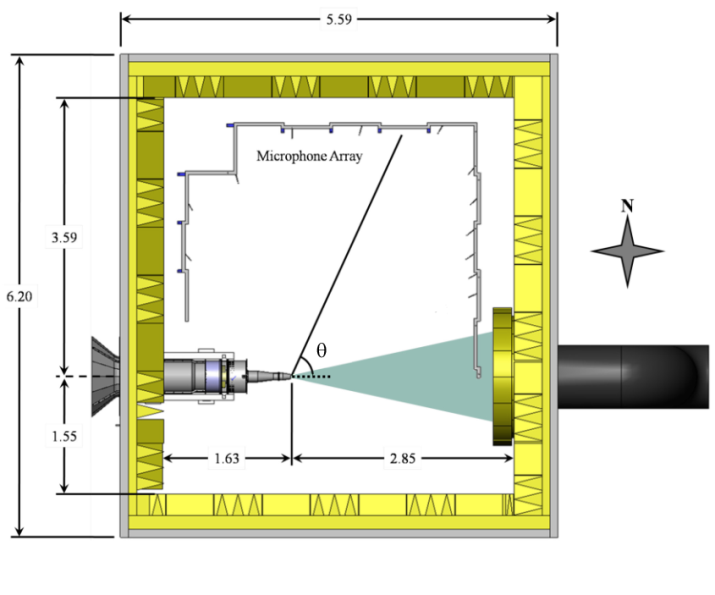
\includegraphics[width=3.5in]{GDTL_facility_schematic.png}
		\caption{Plan view of GDTL free jet facility; dimensions in meters.}\label{GDTLschematic}
	\end{center}
\end{figure}
	
Excitation was applied to jet shear layer via eight LAFPAs which were uniformly spaced around the nozzle perimeter 1 mm upstream of the nozzle exit. Each LAFPA consists of a pair of tungsten pin electrodes with tip spacing (center-to-center) of 4 mm. The electrodes are housed in a boron nitride extension attached to the end of the nozzle.A more detailed description of LAFPA characteristics can be found in Utkin et al. \cite{uyg2007-1}. The LAFPAs are energized by a multi-channel, high-voltage plasma power generator capable of simultaneously powering up to eight LAFPAs, which was designed and built in-house at the GDTL. In the second-generation power supply, each individual circuit consists of a switchable capacitor in line with a high voltage transformer; the arcing electrodes are connected to the secondary side of the coil.The switches are controlled by a 16-channel digital I/O card and National Instruments' Labview software, operated by a dedicated computer. The plasma generator provides independent control of the frequency, duty cycle/pulse width, and phase of each individual actuator (though at a constant amplitude of 5 kV).The pulse width was held constant at 7 $\mu$s, which was found to be the minimum pulse width at which the actuators consistently arced for all frequencies explored in this study \cite{hkfs-2011}. In order to improve our understanding of the linear and nonlinear dynamics of the large-scale structure interactions, the excitation Strouhal numbers ranges from 0.02 to 0.50; an azimuthal mode of $m = 0$ was used in all cases.

Near-field and far-field pressure measurements were acquired simultaneously, using Br�el \& Kj�r 1/4 inch 4939 microphones. The signal from each microphone is band-pass filtered from 20 Hz to 100 kHz using a Br�el \& Kj�r Nexus 2690 conditioning amplifier, and recorded using National Instruments PXI-6133 A/D boards and LabView software. The microphones are calibrated using a Br�el \& Kj�r 114 dB, 1 kHz sine wave generator. The frequency response of the microphones is flat up to roughly 80 kHz, with the protective grid covers removed. Voltage signals are collected at 200 kHz with 81920 data points per block; sub-blocks of 8192 data points were used when calculating short-time power spectral densities, resulting in a frequency resolution of 24.4 Hz. Ten blocks were recorded for each case, resulting in four seconds of data. Analysis of the far-field acoustic spectra found this length to be sufficient for statistical convergence of the turbulence statistics.
\begin{figure}
	\begin{center}
		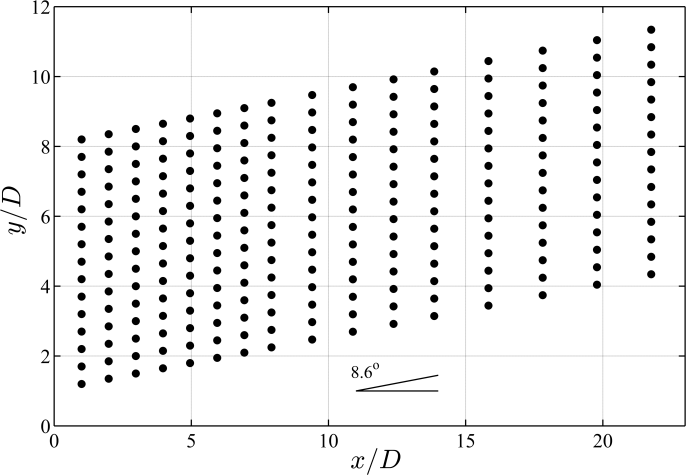
\includegraphics[width=3.5in]{GDTL_mic_locations.png}
		\caption{Near-field microphone array grid.}\label{mic_grid}
	\end{center}
\end{figure}

Far-field acoustic pressure is acquired at three polar angles: 30�, 60� and 90�, as measured from the downstream jet axis. The radial distance of the microphones ranges from 101D at 30� to 145D at 60�. The near-field pressure was acquired using a linear array of sixteen microphones located along the meridional plane of the jet; the spacing varied along the array from 1D to 2D (Fig. \ref{mic_grid}). The linear array is mounted to a traverse system at an angle of 8.6� to the jet axis in order to match the spreading angle of the jet shear layer for this Mach number \cite{kfm2009-1}. The traverse is controlled using LabView and enables the acquisition of pressure measurements at various radial positions with respect to the jet axis. Initially, the most upstream microphone is positioned at x/D = 1 and r/D = 1.20, to ensure that the microphone tips are outside the mixing layer and do not affect the flow field. For subsequent cases, the microphone array is incremented radially outward by 0.5D for a total travel distance of 7D. Signals from the near-field array are preprocessed in order to remove actuator-self noise while retaining the true hydrodynamic and acoustic response of the jet. This has been accomplished via a filter operating in the continuous wavelet domain. Further details may be found in Crawley et al. \cite{Crawley2015}.

\section{Computational Model}\label{theo}
The simulations employ the same approach as previously used
to simulate a Mach~$1.3$ jet without and with
control\cite{gdv2011-POF,SpethCF2013}.  The full compressible
Navier-Stokes equations are solved in curvilinear coordinates
($\xi,\eta,\zeta$) using the
strong conservative form\cite{vm74-1,sjl78-1}. The transformed
non-dimensional equations in 
vector notation are given as: 
\begin{equation}
\frac{\partial}{\partial\tau}\left(\frac{\vec{U}}{J}\right)+\frac{\partial\hat{F}}{\partial\xi}+\frac{\partial\hat{G}}{\partial\eta}+\frac{\partial\hat{H}}{\partial\zeta}=\frac{1}{Re}\left[\frac{\partial\hat{F}_{v}}{\partial\xi}+\frac{\partial\hat{G}_{v}}{\partial\eta}+\frac{\partial\hat{H}_{v}}{\partial\zeta}\right]\label{navier}
\end{equation}
where $\vec{U}=\left\{ \rho,\rho u,\rho v,\rho w,\rho E\right\} $
denotes the solution vector and
$J=\partial\left(\xi,\eta,\zeta,\tau\right)/\partial\left(x,y,z,t\right)$
is the transformation Jacobian.  Details of the various terms in
Eqn.~\ref{navier} may be found in Speth and 
Gaitonde\cite{speth2012b}.
For the inviscid terms, a third-order upwind biased approach is
adopted, together with the Roe scheme\cite{rpl81-1} for flux evaluation.  The
limiter required to enforce monotonicity is a crucial 
component of the method.  The van Leer harmonic limiter\cite{lbv79-1}
has proven to be very successful at reproducing the main features of the
unsteadiness in the jet.  The viscous 
terms are discretized with second-order centered differences and time
integration is performed by a second-order diagonalized~\cite{pth81-1}
approximately 
factored method~\cite{br78-1}.  A sub-iteration
strategy is used to minimize errors due to factorization, linearization and
explicit boundary condition implementation.
\begin{figure}
\begin{center}
	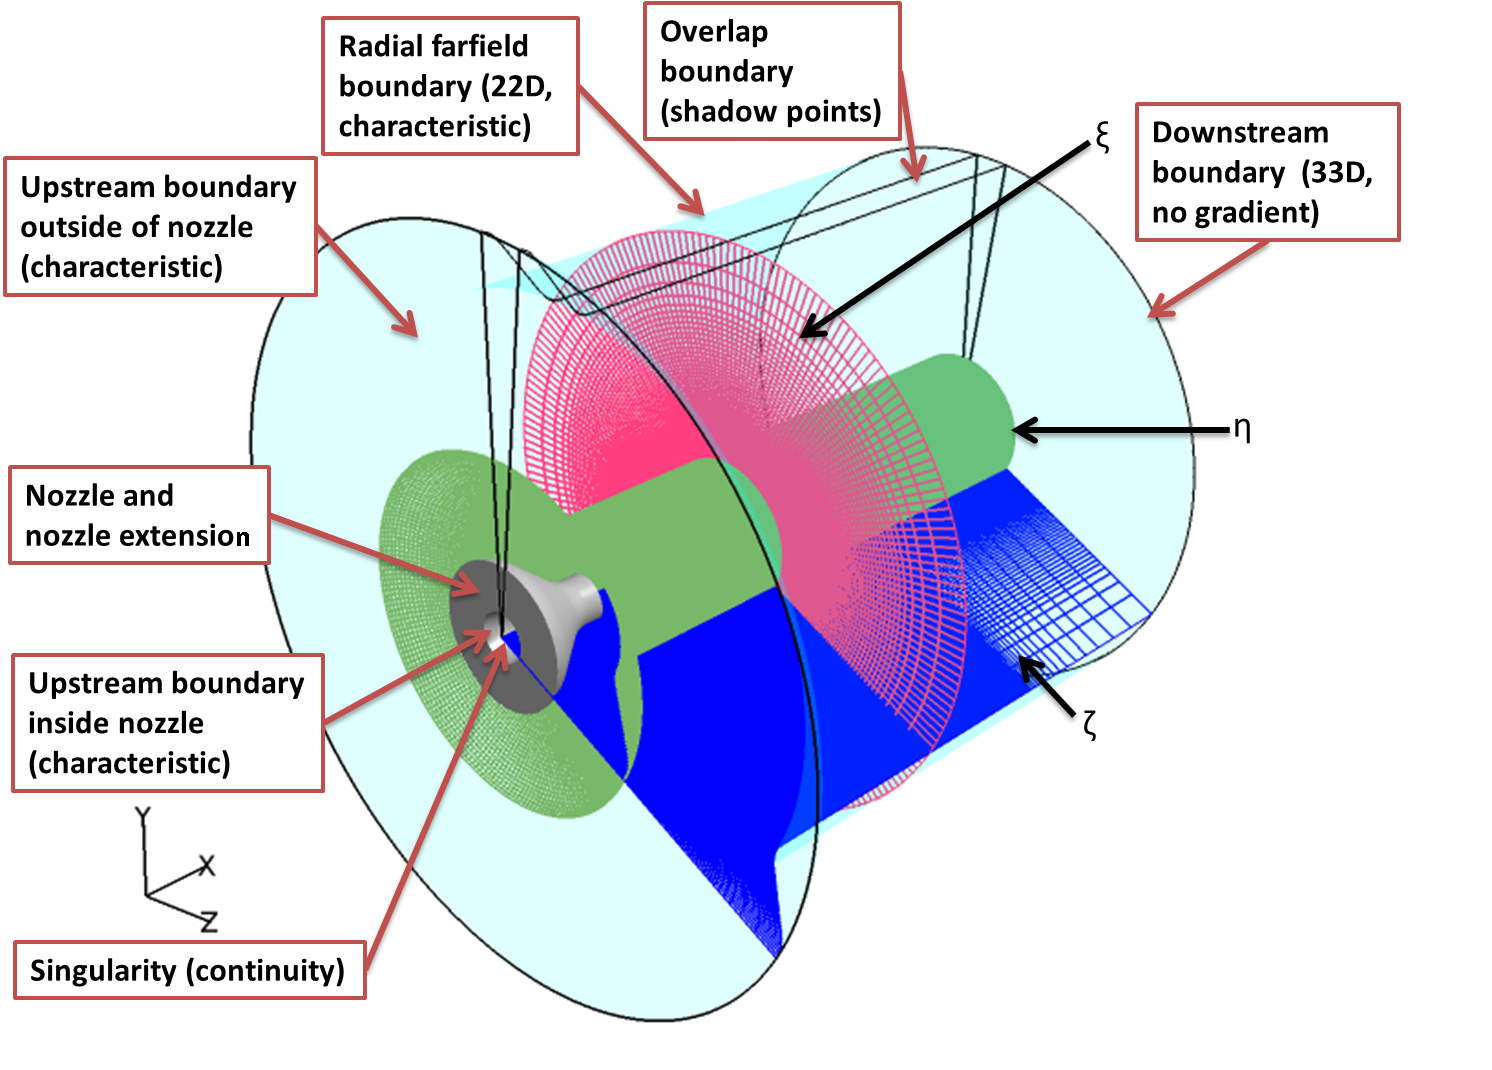
\includegraphics[width=3.5in]{MACH09ComputationalDomain1.png}
\caption{Computational domain}\label{fig:M09Computationaldomain}
\end{center}
 \end{figure}

 A $65$ million point mesh (Fig.~\ref{fig:M09Computationaldomain}) is
 used to simulate the Mach~$0.9$ jet measured in the experiment (Fig.
 \ref{GDTLschematic}).  The grid has dimensions of $685$ points on the
 $\xi$ (streamwise) direction, $455$ points in the $\eta$ (radial)
 direction, and $209$ points in the $\zeta$ (azimuthal) direction. In
 the radial direction, the mesh is refined in the nozzle region and
 gradually stretched in the far field. At the exit of the nozzle, the
 grid maintains a constant axial spacing until after the potential
 core length; then stretches in the streamwise direction as well. To
 preserve continuity, the grid has a five point overlap in the $\zeta$
 direction. Characteristic boundary conditions\cite{bj2000-1} are
 applied to the upstream (outside the nozzle) and radial boundaries.
 Non-reflecting conditions are applied to the downstream and far-field
 boundaries. Stagnation conditions are specified at the first $\xi$
 plane of the nozzle ($\rho_{inlet}=2.04kg/m^{3}$, $U_{inlet}=22m/s$, $P_{inlet}=171,427Pa$) to
 achieve perfectly expanded nozzle exit conditions corresponding to
 $\rho_{jet}=1.404kg/m^{3}$, $U_{jet}=285.99m/s$, $T_{jet}=251.31K$ which match the experiments.
 Based on the nozzle diameter therefore, the Reynolds number is
 $Re=635,308$. The nozzle geometry resembles that of the 
 experiments including the nozzle ring on which the actuators are
 mounted. 
 The velocity profile at the entrance to the nozzle is that
 of a uniform flow (zero at the wall and $U_{inlet}$ everywhere else).
 Perturbations were not introduced into the inflow due to the
 unknown perturbations in the experiment. Therefore, the simulations
 have a laminar boundary layer at the nozzle exit while the
 experiments have a very thin turbulent boundary layer (the momentum
 thickness has been estimated to be $0.09 mm$).  Previous studies have
 shown that despite this difference, the main features of the
 experimental observations are successfully reproduced by the
 computations\cite{gdv2011-POF,SpethCF2013}.  Other studies have shown
 that a smaller $32$ million point simulation is adequate to reproduce
 the features of the experiment\cite{spethASME2013}.

\begin{figure}[h]
\begin{center}
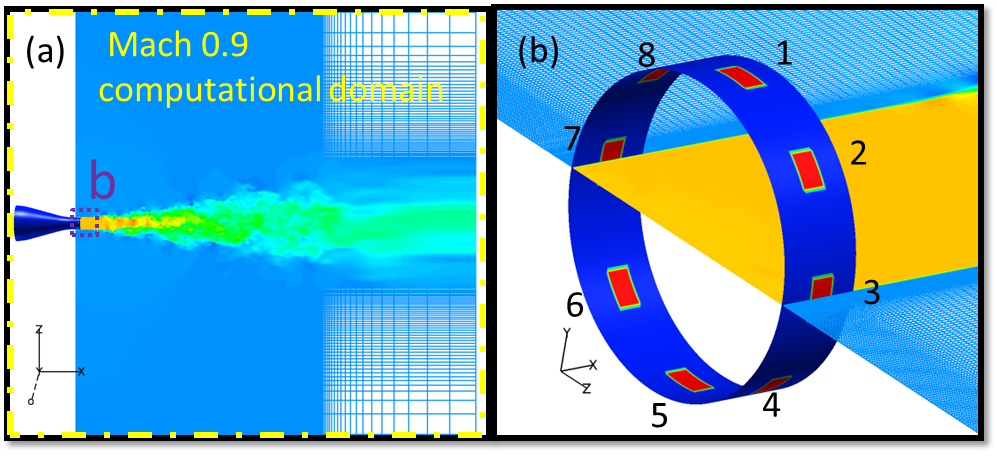
\includegraphics[width=3.6in]{actuatormodelnew}
\caption{The computational domain including the nozzle  (a), and the numerical actuator model (b)}\label{fig:actuator}
\end{center}
\end{figure}
The LAFPAs are modeled after the experiments using a surface heating
technique to excite jet shear layer instabilities and azimuthal modes
within the jet.  Eight actuators are placed around the periphery of
the jet on the nozzle collar at the locations and dimensions of the
experiments as explained previously. As shown in
Fig.~\ref{fig:actuator}b, each actuator consists of a heated region of
the nozzle wall which extends the azimuthal length corresponding to
the separation distance between electrodes ($3 mm$) and has an axial
extent equal to the length of the groove ($1 mm$). The temperature of
the nozzle wall was assumed to be $1.12T_{\infty}$.  When the actuator
is on the temperature of the actuator region increases to
$5T_{\infty}$. Little difference was seen in the previous work (Speth
and Gaitonde\cite{SpethASM2012}) for the temperature range measured in
experiments (Utkin {\em et al.}\cite{uyg2007-2}) for a Mach number of
1.3.  The semi-empirical model is necessary to avoid first-principles
simulation of the poorly understood plasma heating process, as well as
to restrict the required computational resources to feasible levels
(see Ref.~\cite{GaitondeCAF2013-1}).

Unlike acoustic drivers, the LAFPAs are on-off devices and thus can be
represented by rectangular pulses with a duty cycle, which allows for
a wide range of operation choices.  Duty cycle is the percentage of
actuator on time in an excitation cycle. Therefore, a duty cycle
of $100\%$ results in the actuator being on all the time.  
The experimental duty cycle varies with frequency, since the arc
strike lasts a fixed time.  Since the actuator
model is empirical, the computational duty cycle was chosen to obtain
similar control authority as in the experiment.  This necessitates a
higher
duty cycle ($10\%$) than the one used in the experiments
($2.0\%$ for $St_{DF}=0.25$).
As noted earlier, despite the simplicity of the model, its success
has been documented in Gaitonde 
and Samimy\cite{gdv2011-POF}, where, in addition to coherent
structures, mean and fluctuating quantities have been compared.
Furthermore, the mean flow structure with control was shown to match
the theoretical predictions of Cohen and Wygnanski~\cite{cj87-2}.

Like the experiments, the axisymmetric ($m=0$) mode was employed to
study a range of Strouhal numbers. The Strouhal numbers studied in the
simulations include: $0.05$, $0.15$, and $0.25$. Data was acquired
every timestep at the point probes depicted in Fig.~\ref{mic_grid}
as well as on several $\xi$, $\eta$, and $\zeta$ computational planes.
Phase-averaged data were also computed for each of the simulations.

\section{Results}\label{results} 
\subsection{Evolution of the Large-Scale Structures}\label{structure}
The work of Sinha \textit{et al.} \cite{sinha2013} was the first to identify and characterize the temporal signature of large-scale structures in the irrotational near-field of a turbulent, Mach 0.9 jet excited by plasma actuators. They found that each excitation pulse produced a well-defined compact waveform which could easily be recovered from the natural turbulent fluctuations by phase-averaging, a process similar to the triple decomposition of Hussain \& Reynolds \cite{HussainReynolds1970}. When the jet is excited at very low frequencies ($St_{DF} < 0.1$), the characteristic period of the waveform is much shorter than the excitation period. As a result, the structures seeded by the excitation do not interact with one another as they evolve downstream; this behavior was coined the "impulse" response of the jet by the researchers. As the excitation frequency is increased the structures begin interacting, resulting in a periodic waveform with a corresponding reduction of the characteristic structure period and, ultimately, amplitude. Interestingly, it was observed that for moderate excitation frequencies ($St_{DF} \leq 0.5$) this periodic waveform could be well-predicted by a simple linear superposition of impulse waveforms. 

The impulse and periodic phase-averaged waveforms can be observed in Fig. \ref{EXP_Phase_AVG}a, where the the experimental data have been plotted along the first microphone array position at $x/D = 3$, over a large range of excitation frequencies. Here, and throughout the rest of the paper, the pressure has been normalized by the jet dynamic head, $p^{*} = p/\rho_{j} U_{j}^{2} $. Additionally, a linear superposition of the impulse response observed for $St_{DF} = 0.02$ has been plotted against the periodic response observed at $St_{DF} = 0.5$ in Fig. \ref{EXP_Phase_AVG}b. While the waveform shape, temporal extent, and amplitude are all significantly altered from the impulse response, the dynamics which govern the periodic response of the jet in the irrotational near-field behave predominantly in a quasi-linear manner.

\begin{figure}
	\centering{}\subfloat{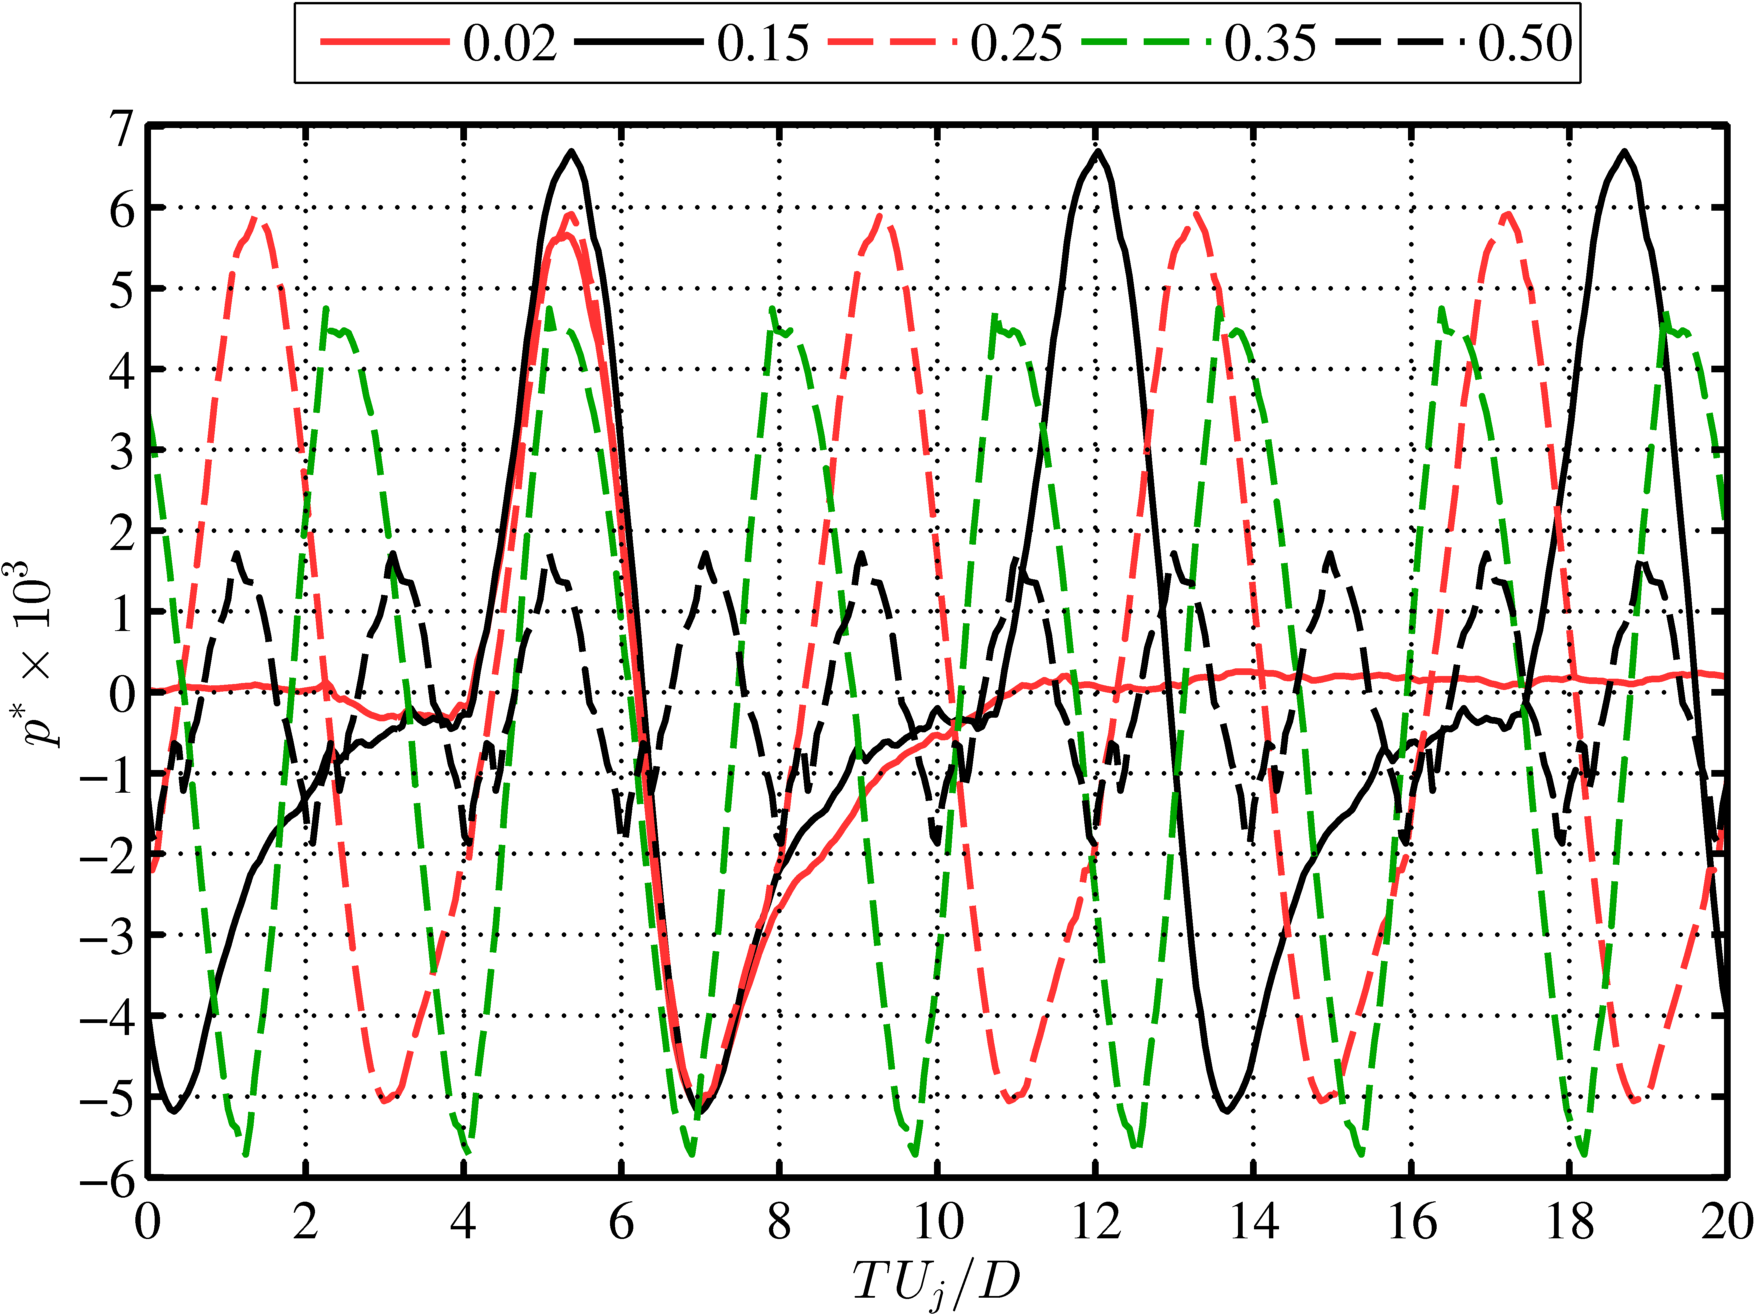
\includegraphics[width=3.25in]{EXP_AP1_x3D_v1.png}
	}\subfloat{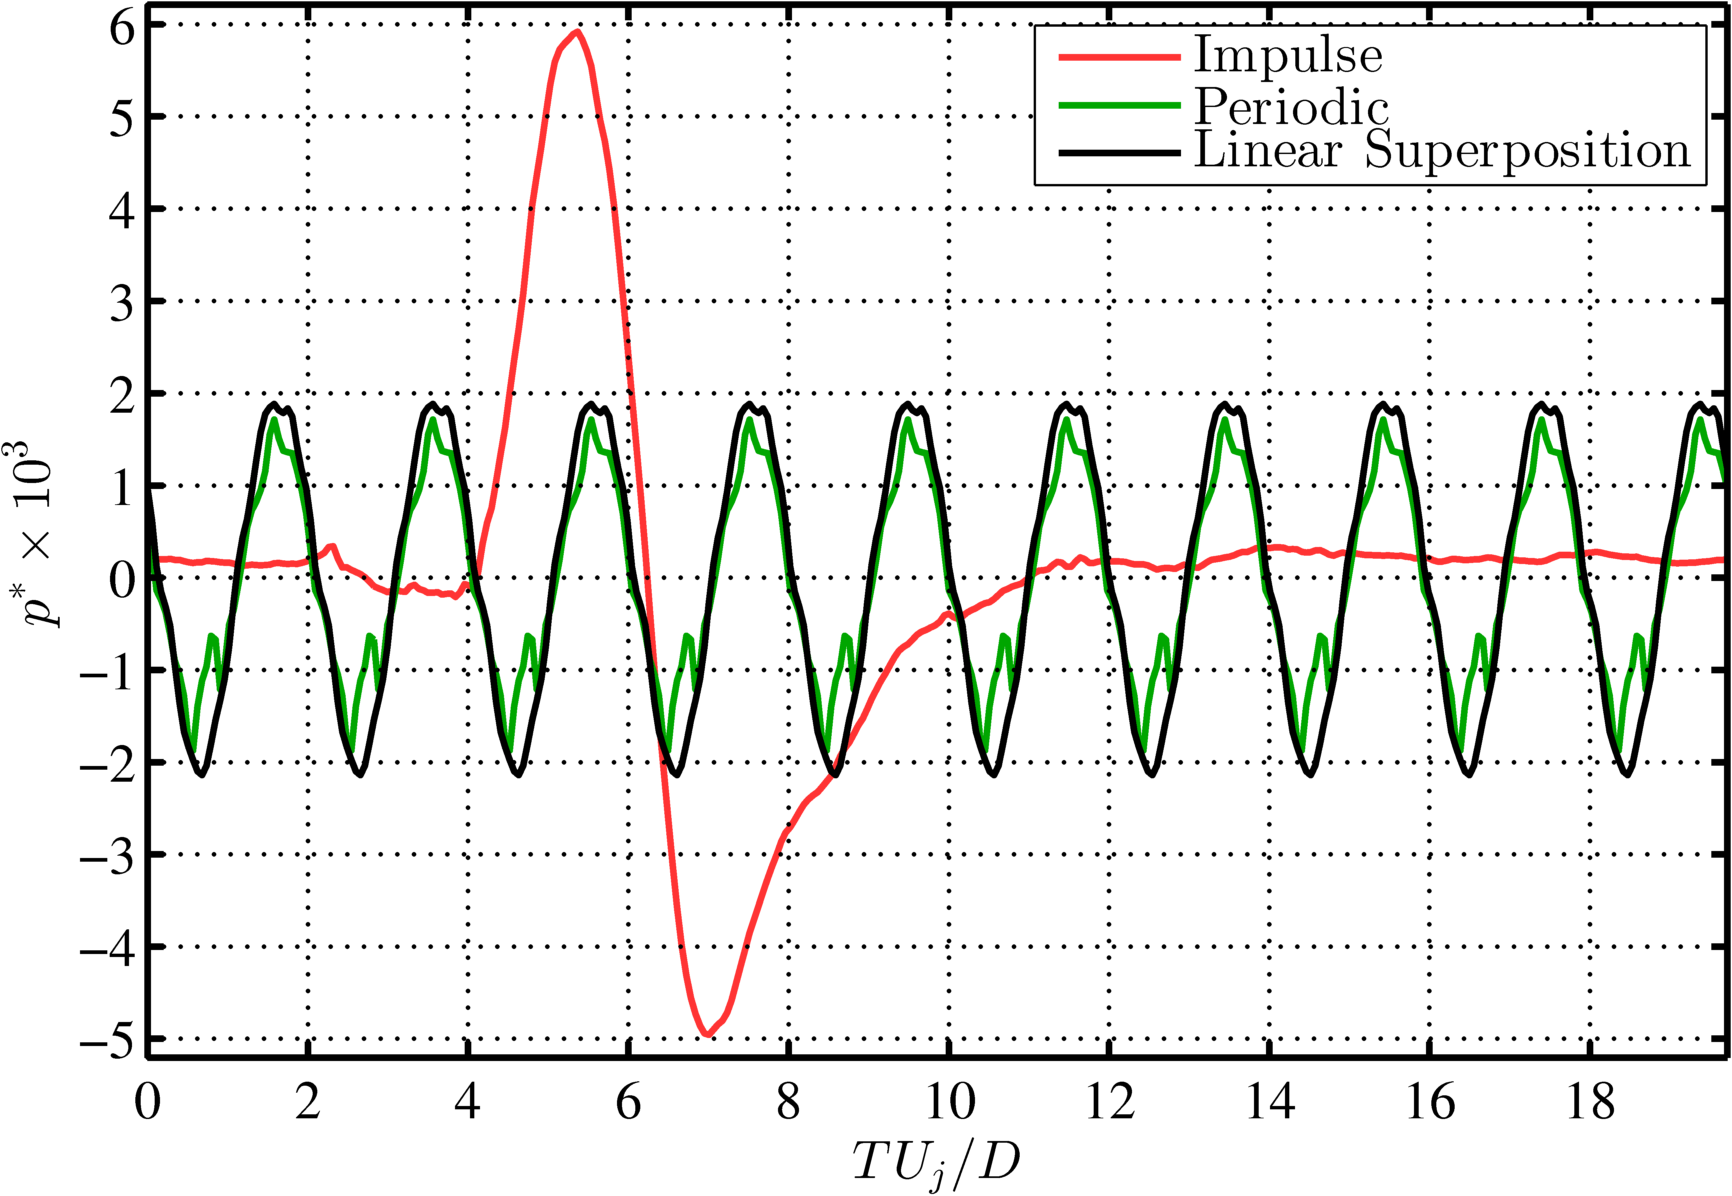
\includegraphics[width=3.25in]{Imp005_Periodic050_total_x3D_v1.png}
}\caption{Phase-averaged waveforms at $x/D = 3$, $r/D = 1.5$ in the experimental database.}\label{EXP_Phase_AVG}
\end{figure}

While the behavior observed in Figs. \ref{EXP_Phase_AVG} sheds new light on the structure evolution and interactions which are ultimately responsible for the acoustic emission, the view provided by the irrotational near-field pressure represents a spatially filtered view of the large-scale structure dynamics due to the strong spatial decay of the evanescent wave produced by the structures \cite{Arndt1997}. Thus, it is desirable to explore directly inside the shear layer in order to get an unadulterated view of the dynamic process by which the large-scale structures transfer energy to the acoustic field. The LES database is indispensable in this regard, as it can provide temporally-resolved, high-fidelity results inside the jet mixing layer, far beyond what is obtainable with current experimental technology.

As a first step, the linear superposition model was evaluated along the jet lipline in the simulated database; this can be seen in Fig. \ref{NUM_Phase_AVG} where the phase-averaged waveforms have been plotted for the same axial location as in Fig. \ref{EXP_Phase_AVG}. Note that there are several differences between the experimental and numerical databases. Foremost among these is the state of the boundary layer as it exits the nozzle. In the experimental jet, the boundary layer has been determined to be fully turbulent \cite{kfm2009-1}. However, the experimental exit profile properties is not available and therefore a the numerical simulations do not included a turbulent exit boundary layer within the nozzle. The sensitivity of the actuated jet response to the exit state and actuator model are currently being studied. Lastly, due to computational
requirements, the simulation time lapse is far shorter than the length of time recorded in the experimental
database; while the phase-averaging occurs over tens of actuation periods in the simulated database, it occurs
over thousands in the experimental.

As a result, it is not expected that the individual waveform shapes or amplitudes will match exactly between the two databases, and indeed they do not: the impulse response observed in Fig. \ref{EXP_Phase_AVG} is quite unlike the impulse response observed in Fig. \ref{NUM_Phase_AVG}. Nonetheless, the linear superposition model still provides good overall match to the periodic response at $St_{DF} = 0.25$, which was the highest frequency explored in the simulations. The waveform shape and amplitude are well predicted by the linear superposition, with one noticeable caveat: the periodic response exhibits dual compression waves. While the linear superposition does produce a secondary compression peak, it is far less prominent. Given the much greater amplitude of the pressure fluctuations along the jet lipline as compared to the irrotational near-field, it is perhaps unsurprising that nonlinear effects play a greater roll. However, the interaction between the structures still appears to be governed predominantly by quasi-linear dynamics.

\begin{figure}
	\centering{}\subfloat{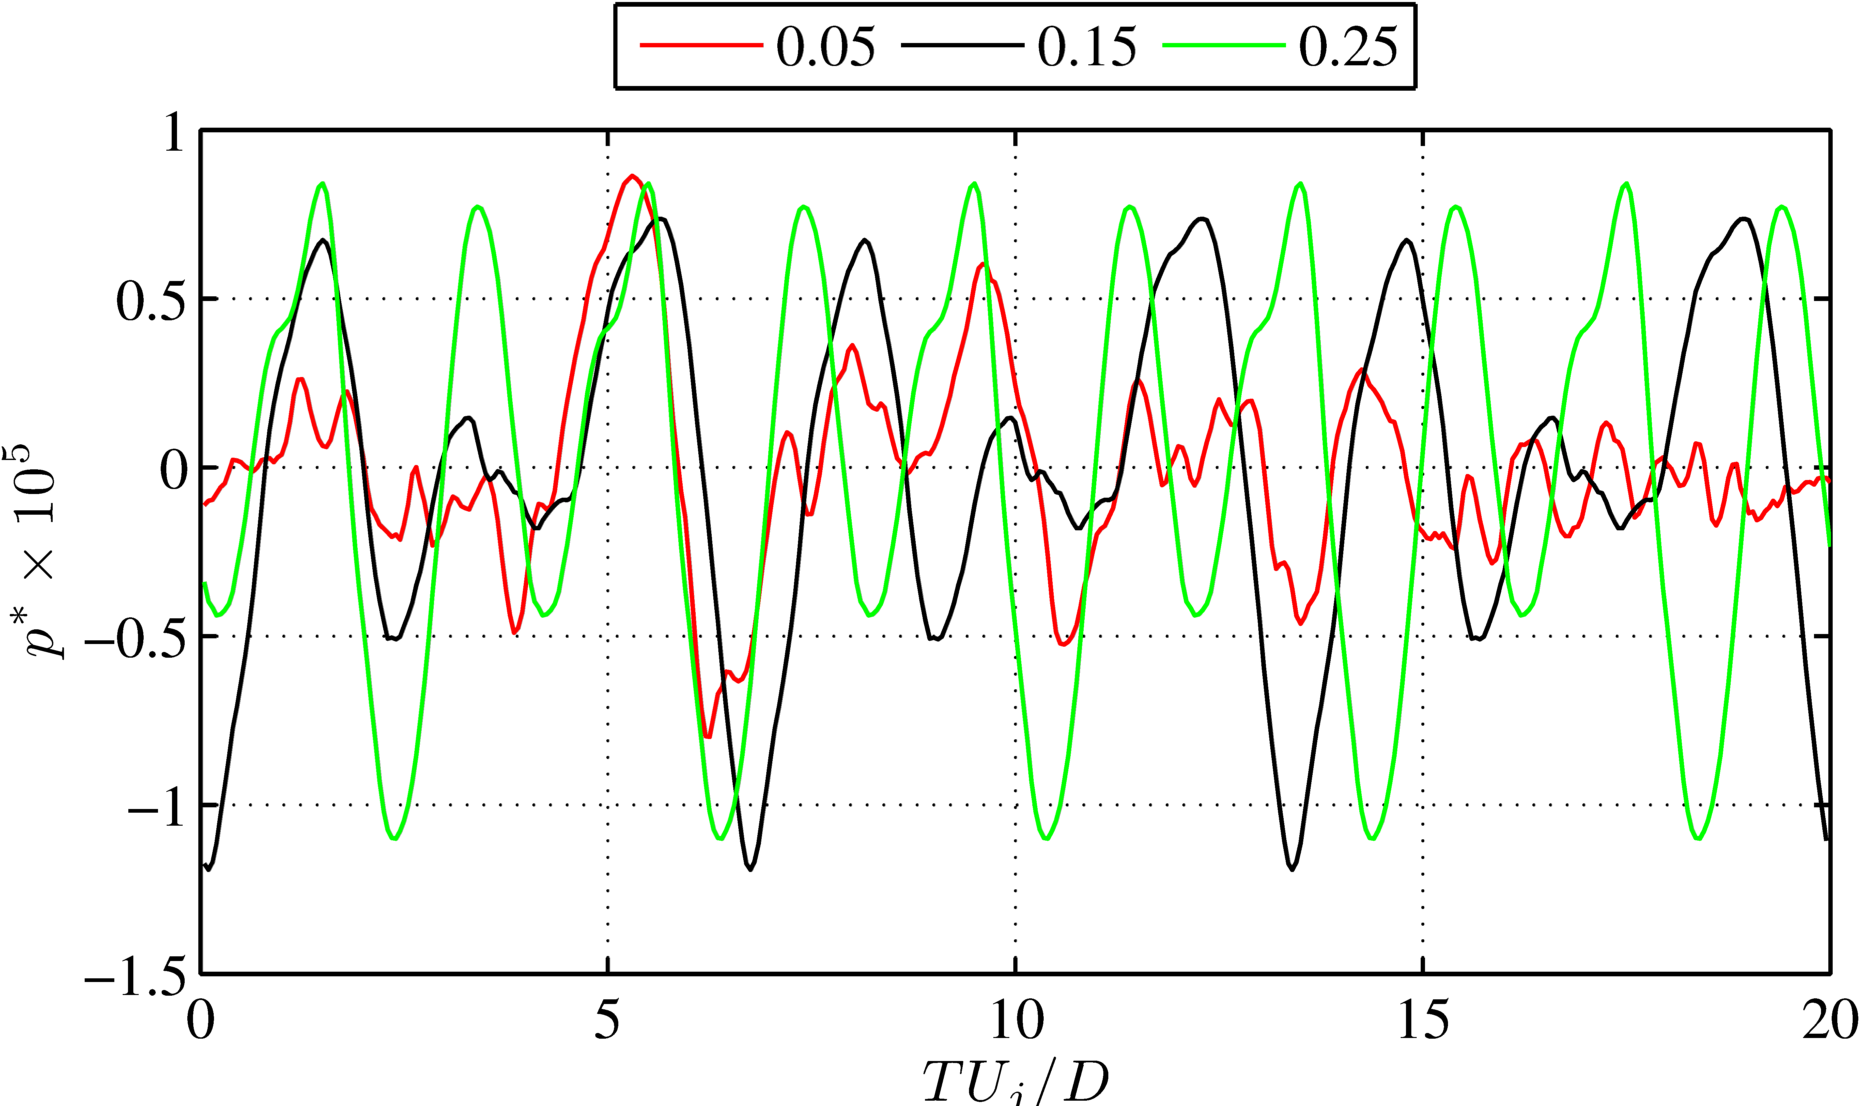
\includegraphics[width=3.25in]{Num_Phavg_x3D_lipline.png}
	}\subfloat{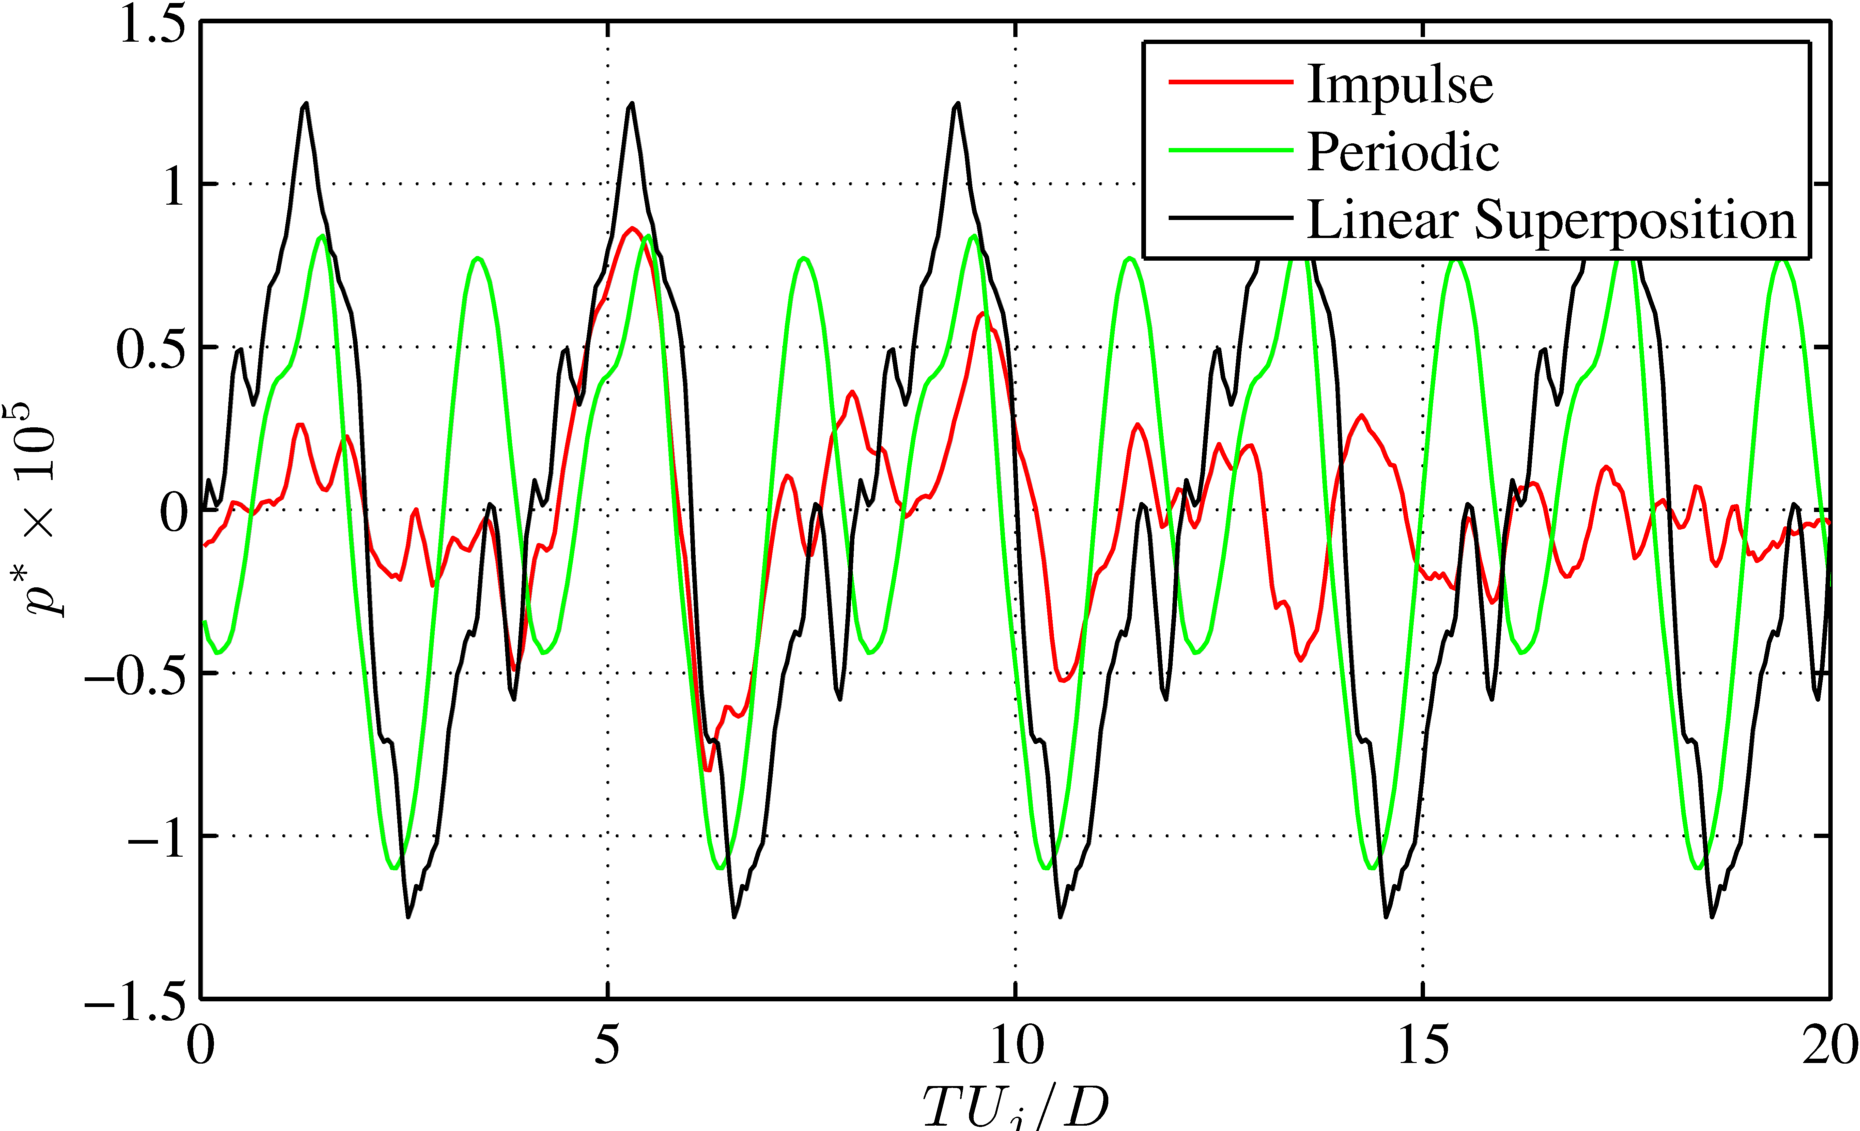
\includegraphics[width=3.25in]{Num_LnrPos_x3D_lipline.png}
}\caption{Phase-averaged waveforms at $x/D = 3$, $r/D = 0.5$ in the numerical database.}\label{NUM_Phase_AVG}
\end{figure}

A broad view of the interactions between the coherent structures generated by the excitation can be easily identified by visualizing isolevels of Q-criterion ($Q=0.35$), colored by axial velocity and overlain on the dilatation field in gray scale. This has been in Fig. \ref{isophase} for $St_{DF} = 0.05$ and $0.25$, using the phase-averaged results. Each figure depicts two phases of the excitation period ($\phi =0.1(2\pi)$ and $0.6(2\pi)$). At each phase, the locations $x/D=2$ and $4$ of the first array are labeled.  For the $St_{DF}=0.05$ cases (Fig.~\ref{isophase}a), the A' and A structures are depicted at phase $0.1(2\pi)$. At phase $0.6(2\pi)$, the structure observed during the first phase has already broken up resulting in no observable actuator induced structures at this phase for this Strouhal number.

Figure~\ref{isophase}b depicts the isolevels of the high frequency ($St_{DF}=0.25$) case. Rollers develop due to the excitation that grow and interact with other actuator induced structures as they propagate downstream. Initially, the structures that are produced at phase $\phi=0.6(2\pi)$ of Fig.~\ref{isophase}b are similar to those associated with the impulse response (Fig. \ref{isophase}a). However, as each structure grows and propagates downstream, it interacts with the structure generated during the prior actuator on event. Thus structures B and B' are equivalent to A and A' respectively, but belong to the previous/subsequent actuator pulse. Since the reaction to the actuation is cyclic, the structures seen at the end of the potential core at one phase ($\phi=0.1(2\pi)$) begin to develop at similar phases in the next cycle. Structure B/A' in phase $\phi=0.1(2\pi)$ occurs when structures B and A' influence each other through self and induced effects. This compression occurs due to the relatively high convective velocity of B (which is closer to the nozzle exit where the speed is higher) compared to A'. This interaction is quasi-linear, creating a sine-like response in the near-field pressure through linear superposition of the two actuator structures (B and A'). 

The structures affect the near-field as seen by the strong dilatation waves surrounding each large scale structure.  The dilatation values
of Fig.~\ref{isophase} may be connected to the pressure profiles of Fig.~\ref{NUM_Phase_AVG}. The white dilatation waves (lower dilatation
value) correspond to an increase in pressure while the black dilatation waves (higher dilatation value) correspond to a decrease in pressure. These pressure fluctuations can be readily seen in the phase-averaged pressure probes along the first array. At a phase of $\phi=0.1(2\pi)=36^\circ$ in Fig.~\ref{isophase}b, the $x/D=4$ point probe is entering a white dilatation region (increase of pressure) while the x/D=2 probe is entering a black dilatation wave corresponding to a decrease in pressure. 

\begin{figure}
	\centering{}\subfloat[$St_{DF}=0.05$]{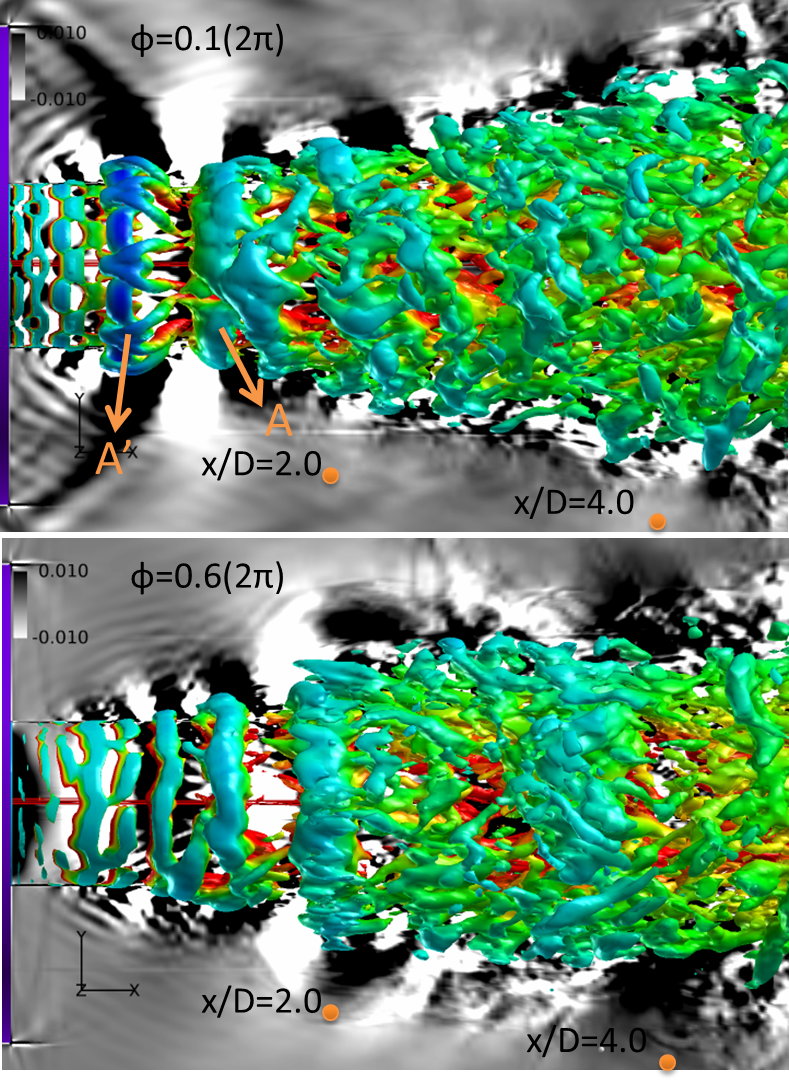
\includegraphics[width=2.9in]{M09St005qcritphase0106AB}
	}\subfloat[$St_{DF}=0.25$]{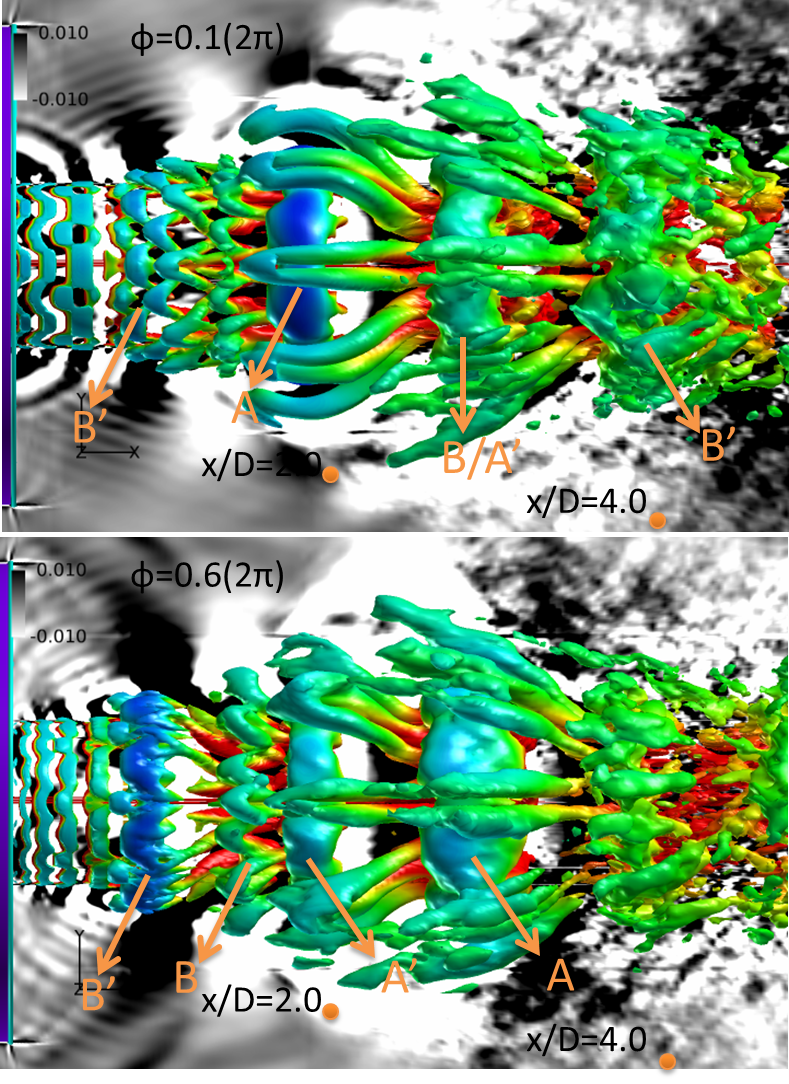
\includegraphics[width=2.9in]{M09St025qcritphase0106AB}
	}\caption{Simulations of the phase avergaered iso-levels of Q-criterion colored by axial velocity with gray scale of dilatation}\label{isophase}
\end{figure}

While these structures cannot be compared directly to the turbulence of the natural jet owing to the lack of a phase-reference, the evolution of the fluctuation intensity (mean-squared pressure, $P_{ms}$) can serve as a simple, if coarse, metric for comparison between the natural and excited structures. The results for the experimental and numerical databases are shown in Fig.~\ref{pms} along the first pressure probe array for the different excitation Strouhal cases and the natural jet (0.00). Similar trends are found for the simulated database, which is not shown here for brevity, though quantitative differences exist for each Strouhal number. The mean square pressure increases with increasing excitation Strouhal number until the column mode Strouhal number is reached ($St_{DF} \simeq 0.3$) at which point the mean square pressure starts to decrease with increasing excitation Strouhal number. Although the computations do not consider Strouhal numbers higher than the most amplified column mode value, we note that in an earlier numerical study a similar reduction in control authority was observed at higher excitation frequencies \cite{SpethCF2013} and the near field pressure fluctuations were also diminished \cite{GaitondeJPropPower2012}. For both experiments and simulations, increasing the excitation Strouhal number also yields an upstream shift in the saturation location.  In the case of the unforced jet, the fluctuations peak at x/D = 5, just upstream of the end of the potential core, and slowly decays beyond that point. Excitation at the lowest frequencies, where the structures do not undergo significant quasi-linear interactions, results in an amplification of the fluctuation energy over nearly the entire domain, though it is most significant near the saturation point. In this case, the saturation point has shifted upstream, to x/D = 4, and displays a slightly sharper peak. These results are consistent with those of other researchers, who have shown that perturbations of higher frequencies saturate earlier upstream than lower frequencies \cite{Suzuki2006,Ukeiley2004}.

\begin{figure}
	\centering{}\subfloat[Experiment]{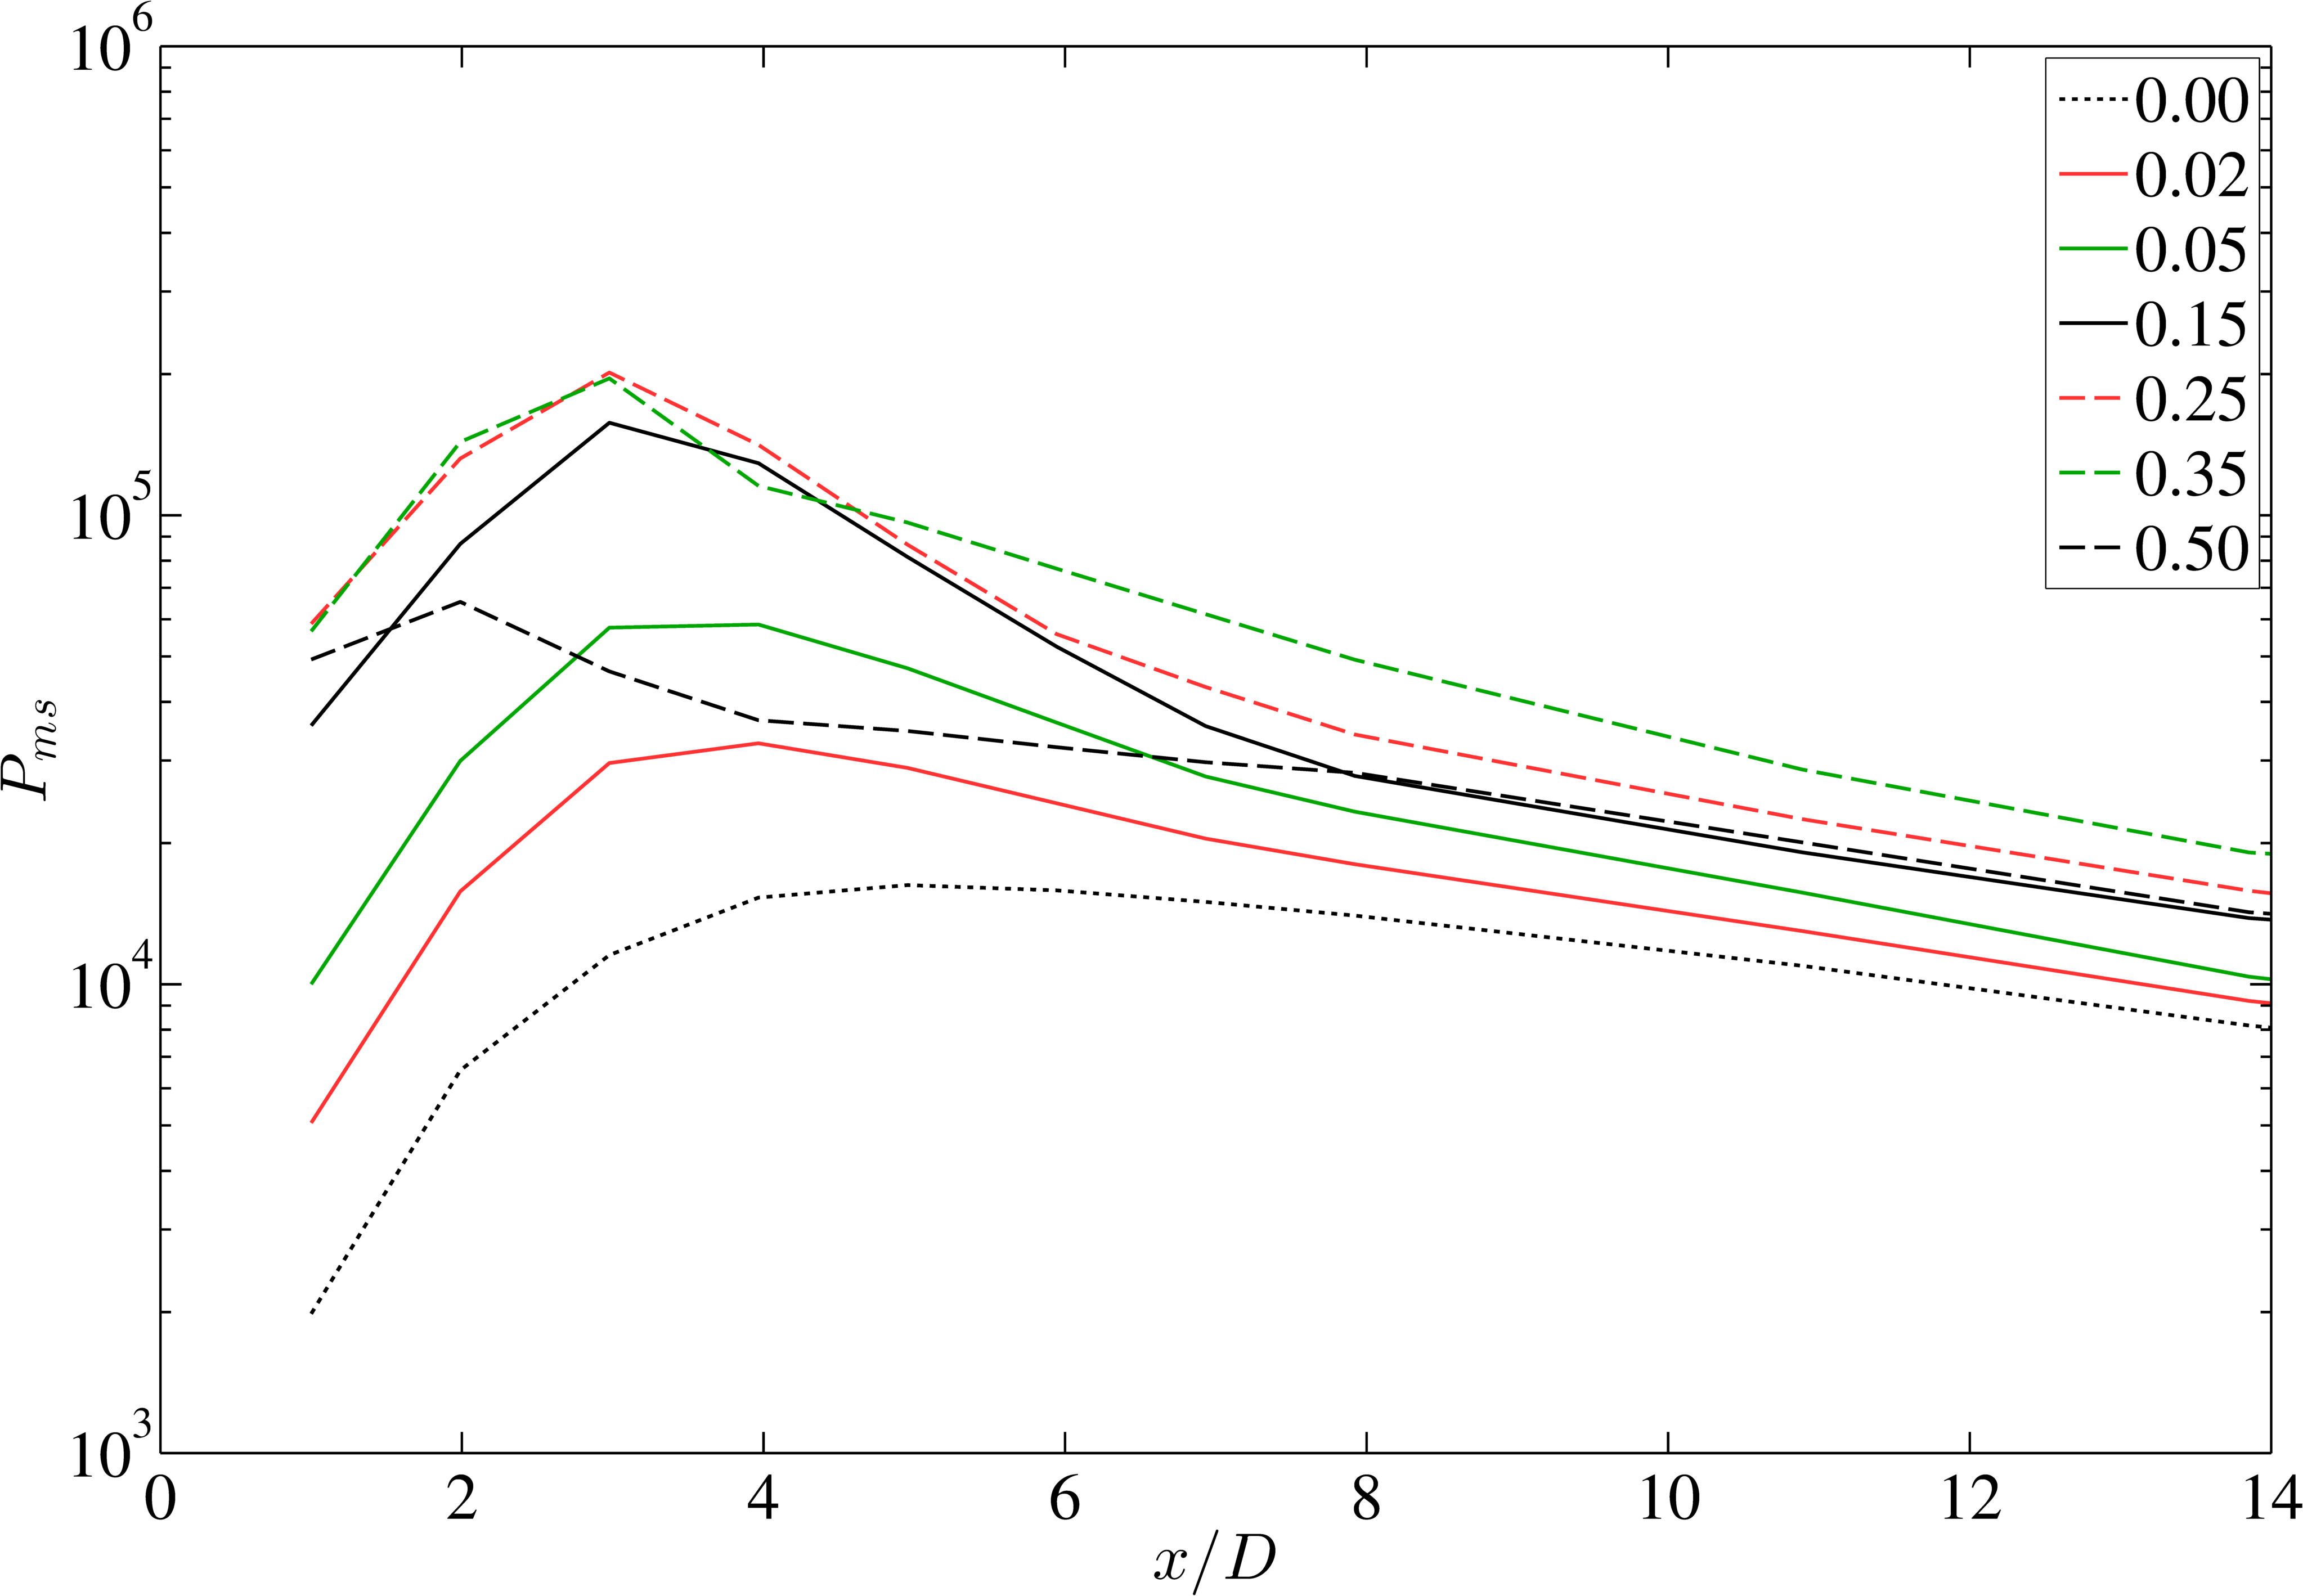
\includegraphics[width=3.25in]{ExpTotalPms.png}}\subfloat[Computations]{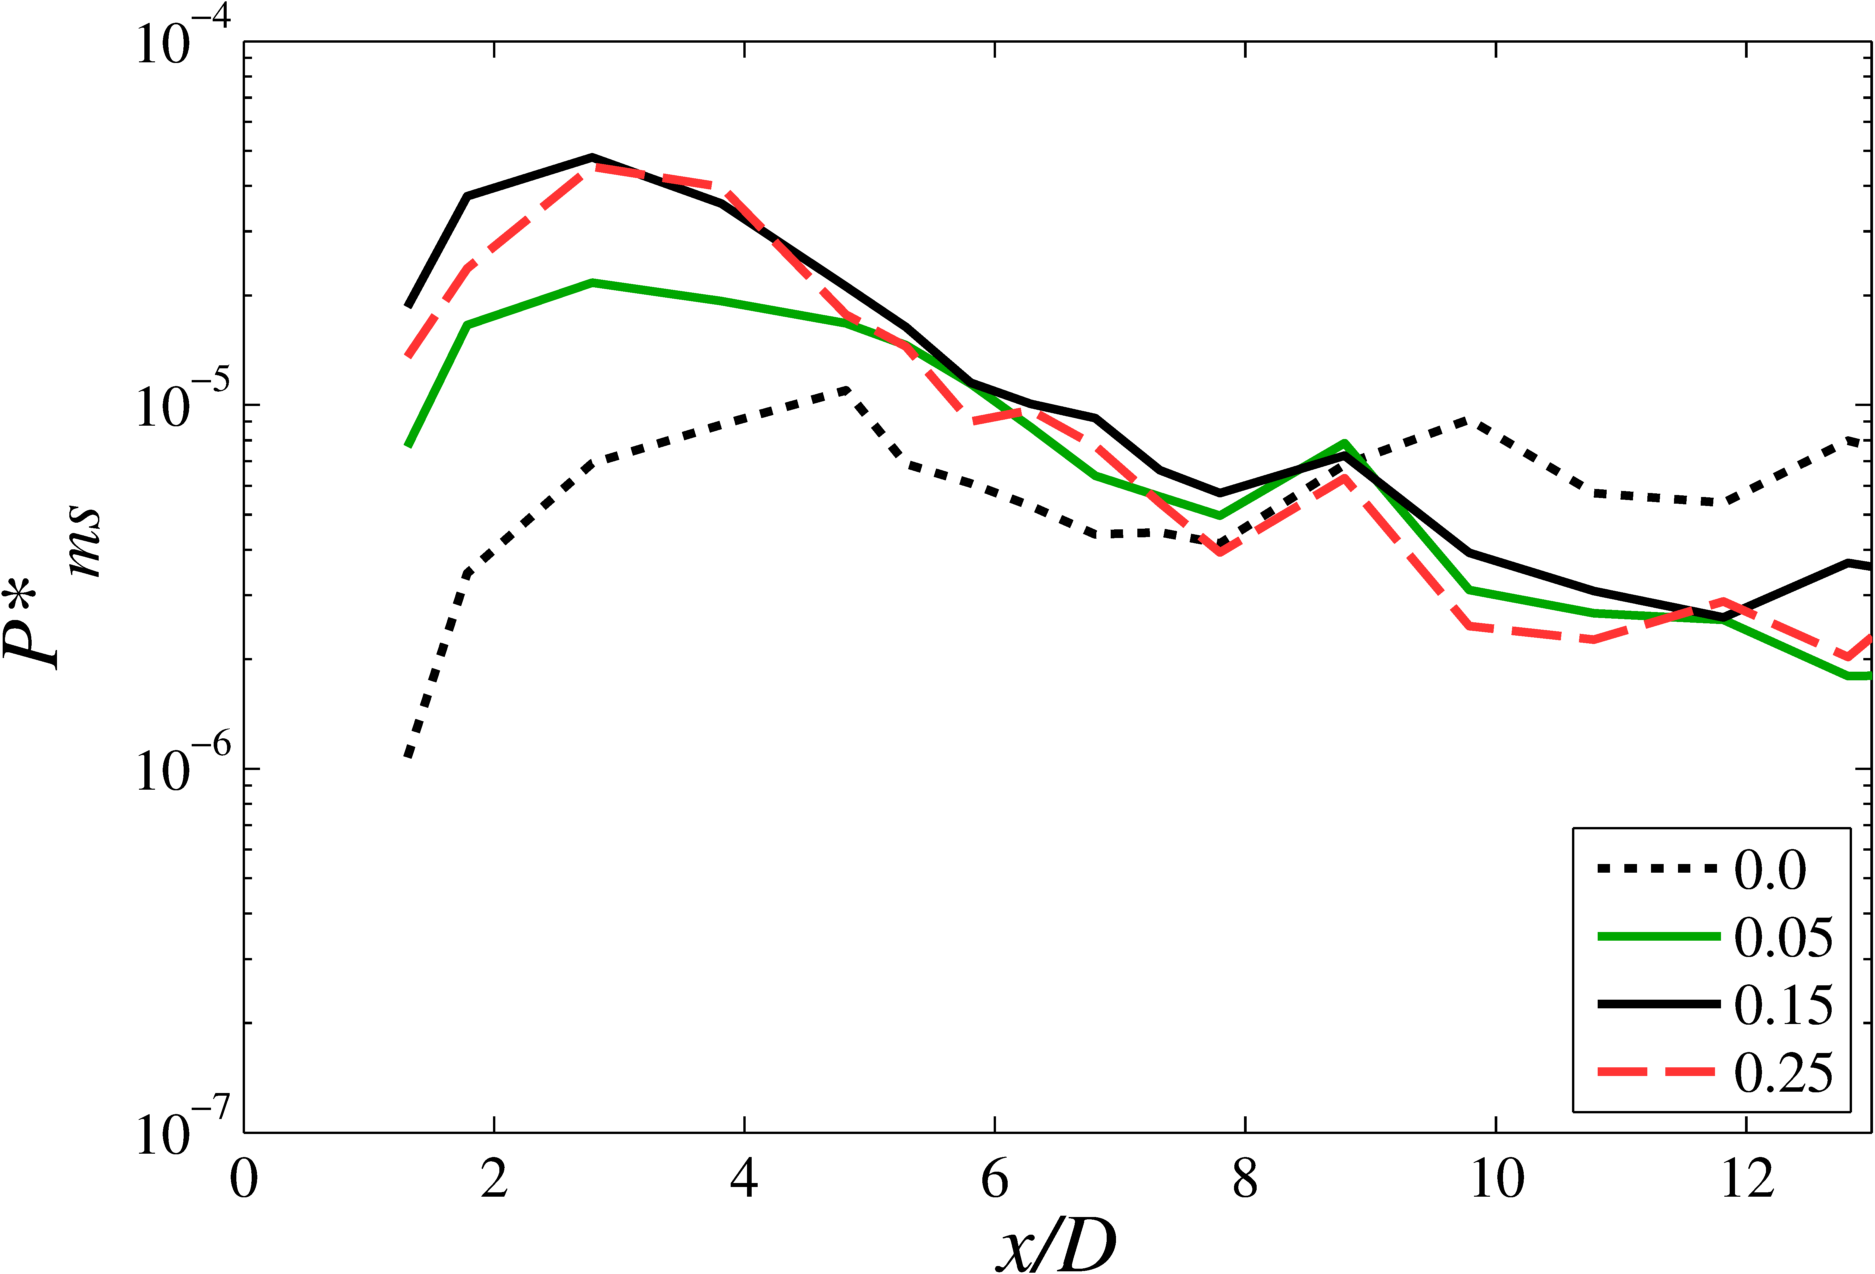
\includegraphics[width=3.25in]{Num_Pms}}
	\caption{Mean-square pressure along the first array (first probe located at $r/D=1.2$)}\label{pms}
\end{figure}

\subsection{Identification of the Acoustic Response}\label{acoustic}
In Crawley \textit{et al.}\cite{Crawley2015} the work of Sinha \textit{et al.}\cite{sinha2013} was extended to the acoustic far-field, where it was found that the excitation again produced a coherent response in the pressure field, and a linear superposition of the impulse response again well-predicted the periodic response, at least at aft angles. This behavior is demonstrated in Fig.~\ref{EXP_FF} for a polar angle of $30^{o}$ in the experimental jet. As with the irrotational near field (which is dominated by hydrodynamic fluctuations), the acoustic far field exhibits a compact waveform for the lowest excitation Strouhal numbers. The behavior of the far-field response did diverge from the near-field in one distinct metric: in the case of the far-field response the linear superposition model was able to predict the periodic response only up to $St_{DF}= 0.25$. The reason behind this is currently not well understood - nonlinear dynamics may become significant to the acoustic emission process beyond this frequency, or the structures at this frequency are no longer radiating efficiently (the far-field spectra peaks around $St_{DF}= 0.15$) and hence are lost in the phase-averaging process.

\begin{figure}
	\centering{}\subfloat[]{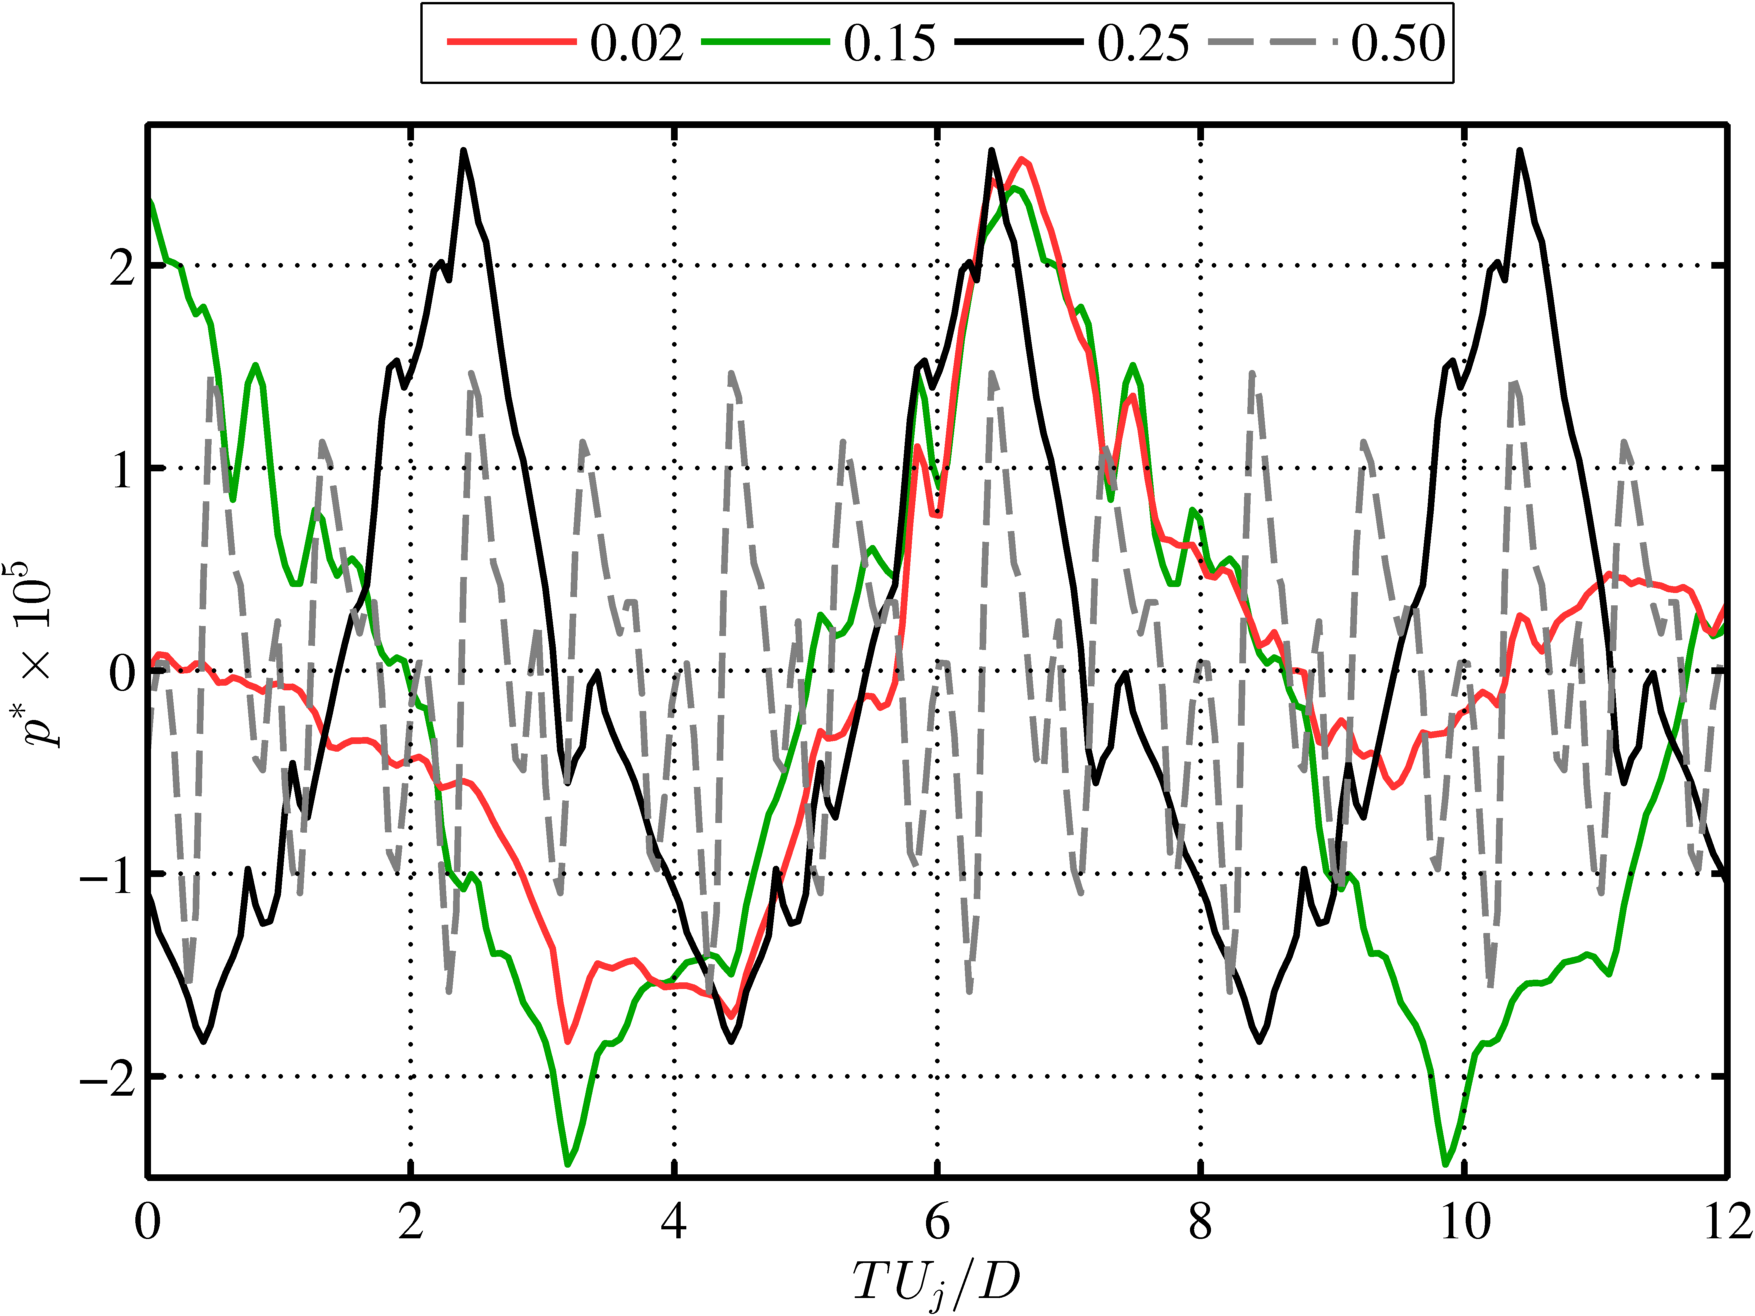
\includegraphics[width=3.25in]{EXP_FFx1.png}}\subfloat[]{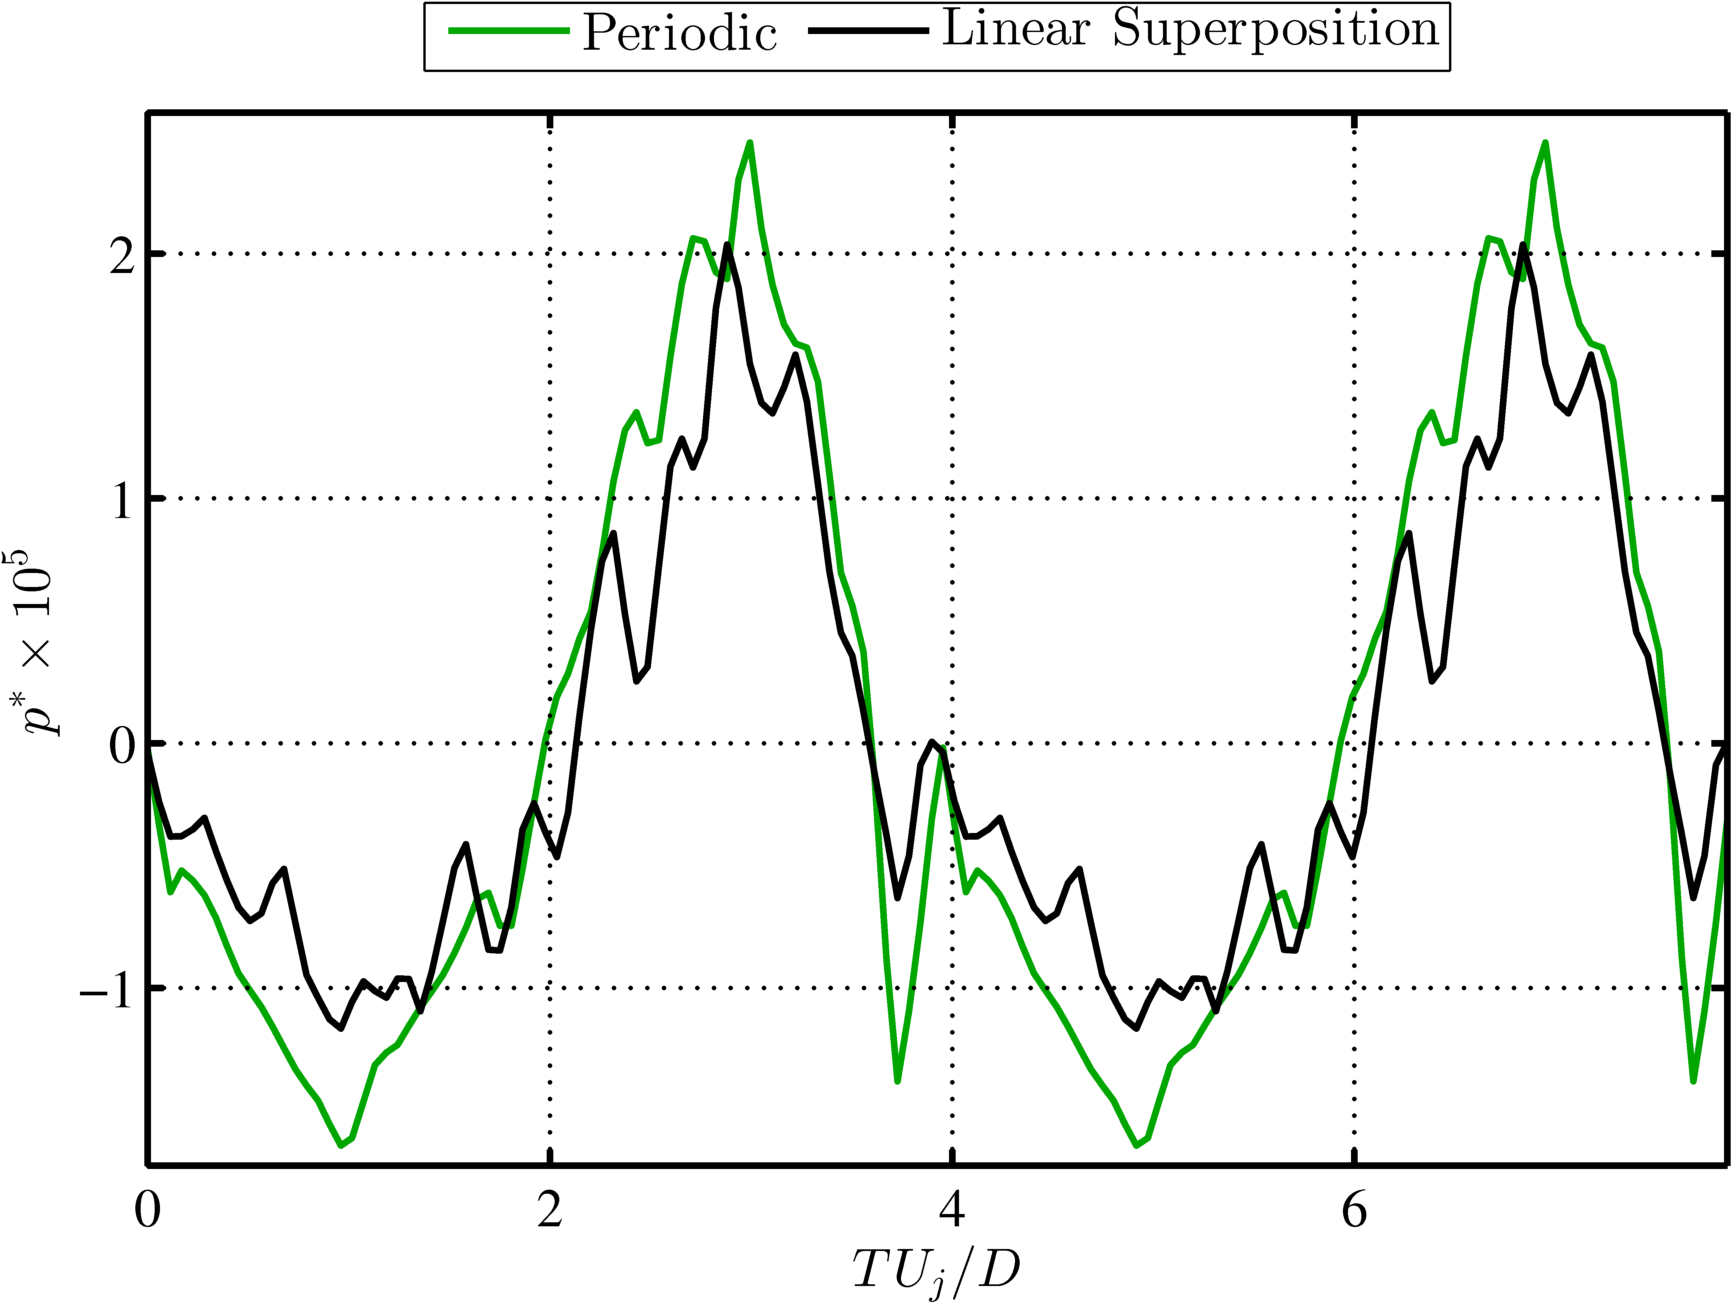
\includegraphics[width=3.25in]{EXP_FFx1_LnrPos.png}}
	\caption{Far-field response to excitation at $30^{o}$ in the experimental jet, phase-averaged waveforms (a) and linear superposition of the impulse response ($ St_{DF}= 0.02$) against the periodic response at $ St_{DF}= 0.25$.}\label{EXP_FF}
\end{figure}

In order to identify the origin of the far-field acoustic emissions (both spatial and temporally), a decomposition of the near-field is desired, as the strong hydrodynamic pressure fluctuations associated directly with the passage of coherent structures largely mask the resultant weak acoustic radiation. As has been shown by Arndt \textit{et al.}\cite{Arndt1997},the irrotational near field of the jet comprises both the hydrodynamic footprint of the large-scale structures in the mixing layer as well as acoustic radiation. The analysis of Coiffect \textit{et al.}\cite{Coiffet2006} showed that the total near field can be thought of as a linear superposition of the hydrodynamic and acoustic fields. Therefore, a suitably designed linear filter can, in principle, extract the constitutive fields from the experimentally measured near field. 

This was first done experimentally by Tinney \& Jordan\cite{Tinney2008}, using a linear array of microphones and a wavenumber-frequency filter in the Fourier domain to separate the irrotational near-field into subsonically- and supersonically-convecting waves. The author's justification for this algorithm was that in an unheated subsonic jet, the hydrodynamic pressure fluctuations will be aligned with the jet axis, and travelling subsonically. Acoustic pressure fluctuations will impinge on the linear microphone array at oblique angles and therefore will appear as having either sonic or supersonic phase velocity based on the source location. In the current work a similar method is used, though the two-dimensional Fourier transform has been replaced with a spatio-temporal wavelet transform. Sample results for this decomposition can be found in Fig.~\ref{EXP_DECOMP} for the experimental database. Here, the full near-field pressure and the acoustic component of the irrotational near-field have been plotted against the far-field acoustic, in the spectral domain in the case of the natural jet and with phase-averaged waveforms in the jet excited at $ St_{DF}= 0.02$. The near-field signals were scaled in amplitude based on the propagative distance from the near-field microphone ($x/D = 8, y/D = 2.2$) in order to account for spherical propagation of the waves. This requires an assumption on the acoustic source region, which is not know with certainty. For the current work, the noise source location was assumed to be centered around $x_{s}/D = 4, y_{s}/D = 0$; the reasoning for this assumption will become more clear in short order.

The decomposition method accurately reproduces the high-frequency content acoustic spectrum, which is unsurprising given that the near-field spectra are dominated by acoustic fluctuations over this range of frequencies (though this does reinforce the accuracy of the amplitude-scaling explained previously). In contrast, the acoustic spectral peak is masked in the near-field by the far more dominant hydrodynamic field. Though imperfect, the decomposition does a good job capturing the peak amplitude, frequency, and low-frequency decay of the true acoustic field. The impulsive excitation provides an additional opportunity to validate the decomposition, this time in the temporal domain. Phase-averaged waveforms for the far field, full near field and acoustic near field have also been analyzed in Fig.~\ref{EXP_DECOMP}b for the jet excited at $St_{DF}= 0.02$. Again, the filtered acoustic signal does differ somewhat from the far-field acoustic signal. However, the overall agreement is remarkable, particularly considering the waveform amplitude and shape differs significantly from the full near-field signal. Clearly, the decomposition algorithm is preserving not only the spectral content but statistically non-stationary events in the acoustic near field. Additional details of the decomposition algorithm and validation in the experimental database can be found in Crawley \& Samimy\cite{crawley2014b}. 

\begin{figure}
	\centering{}\subfloat[]{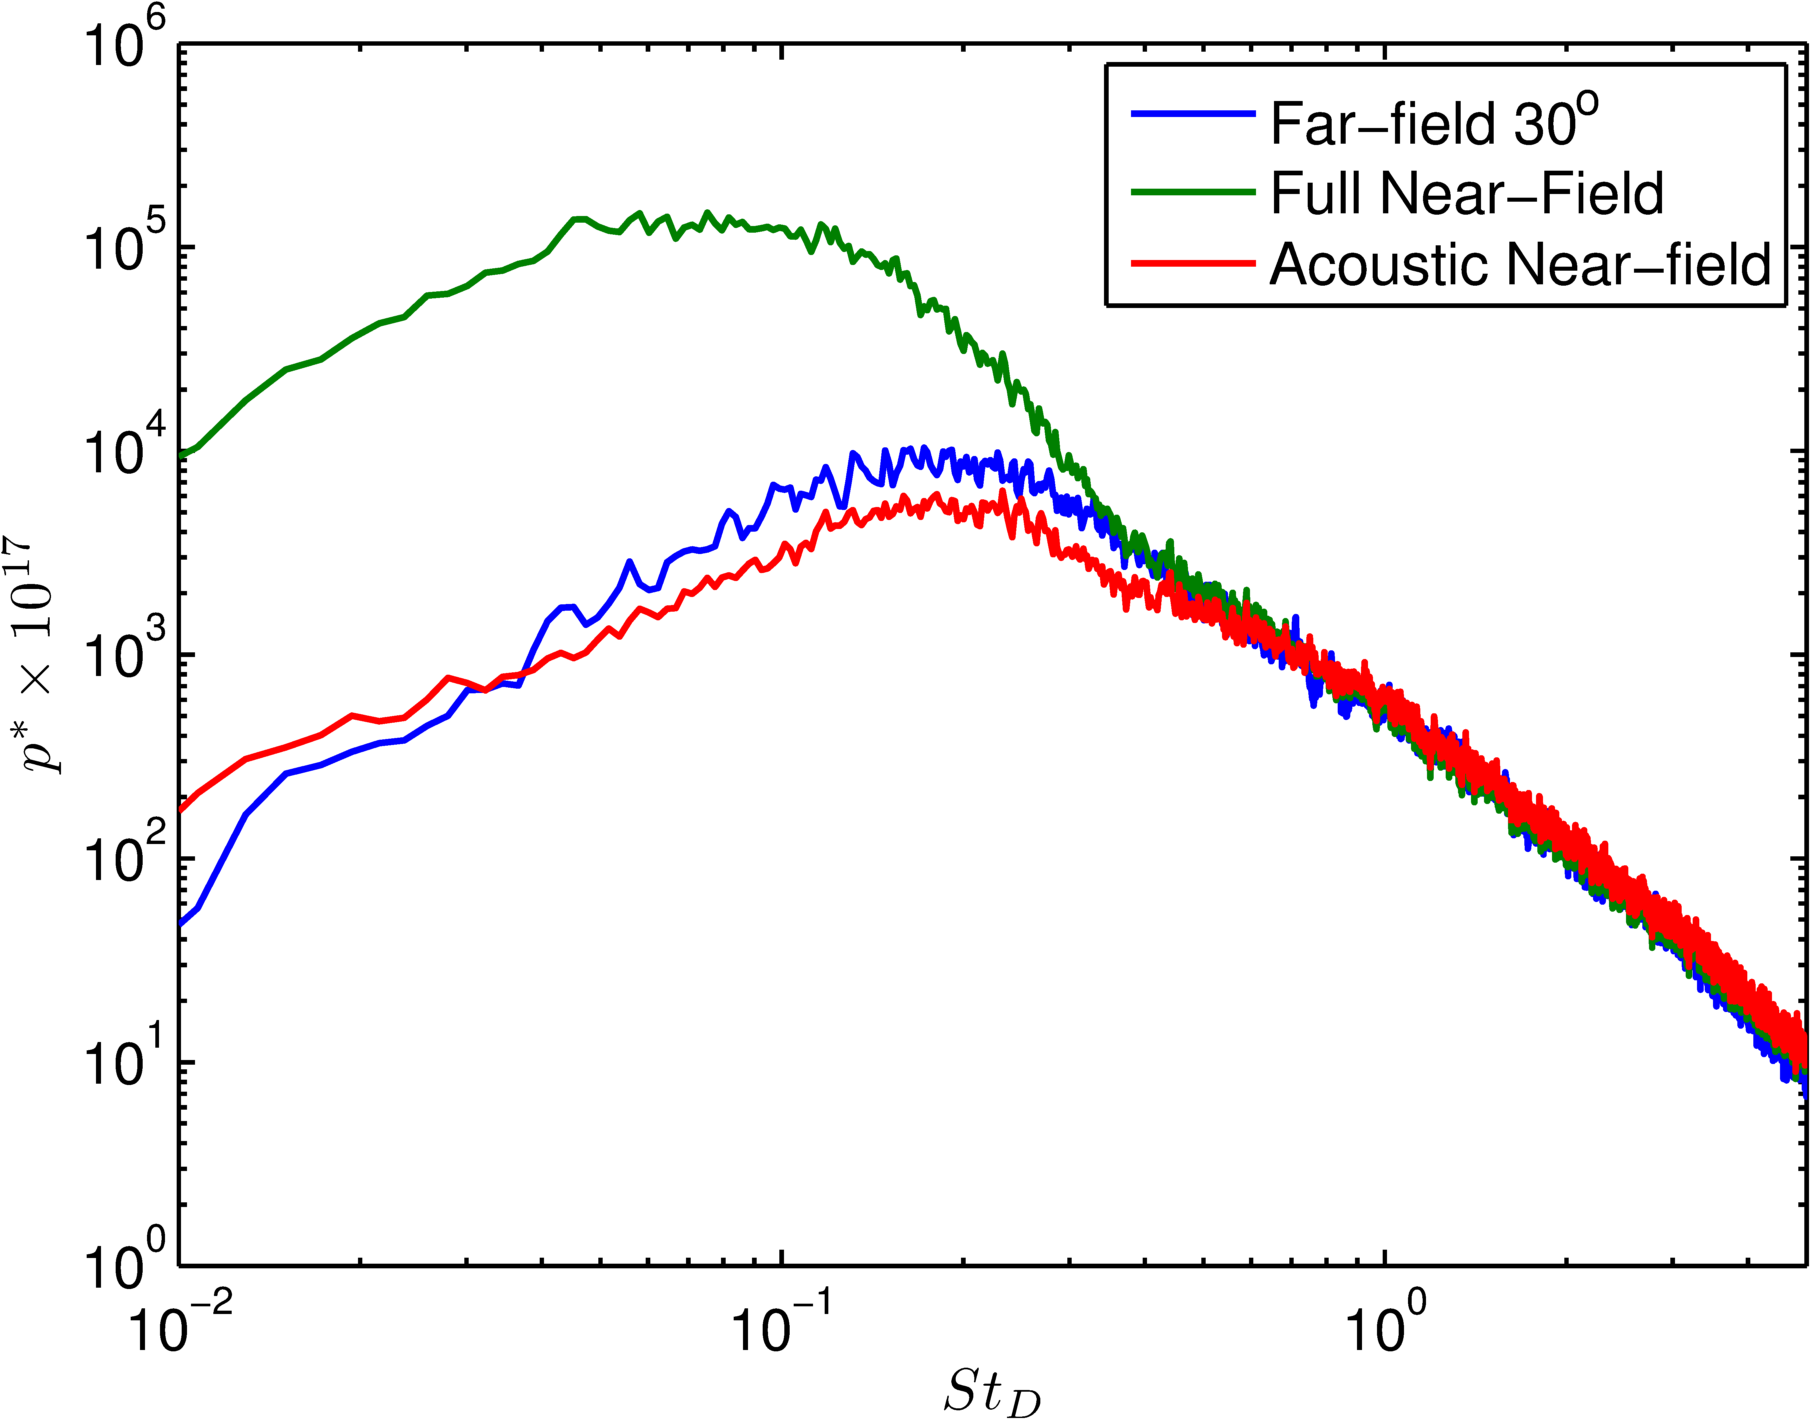
\includegraphics[width=3.25in]{EXP_DECOMP_NFvFF_Spectra.png}}\subfloat[]{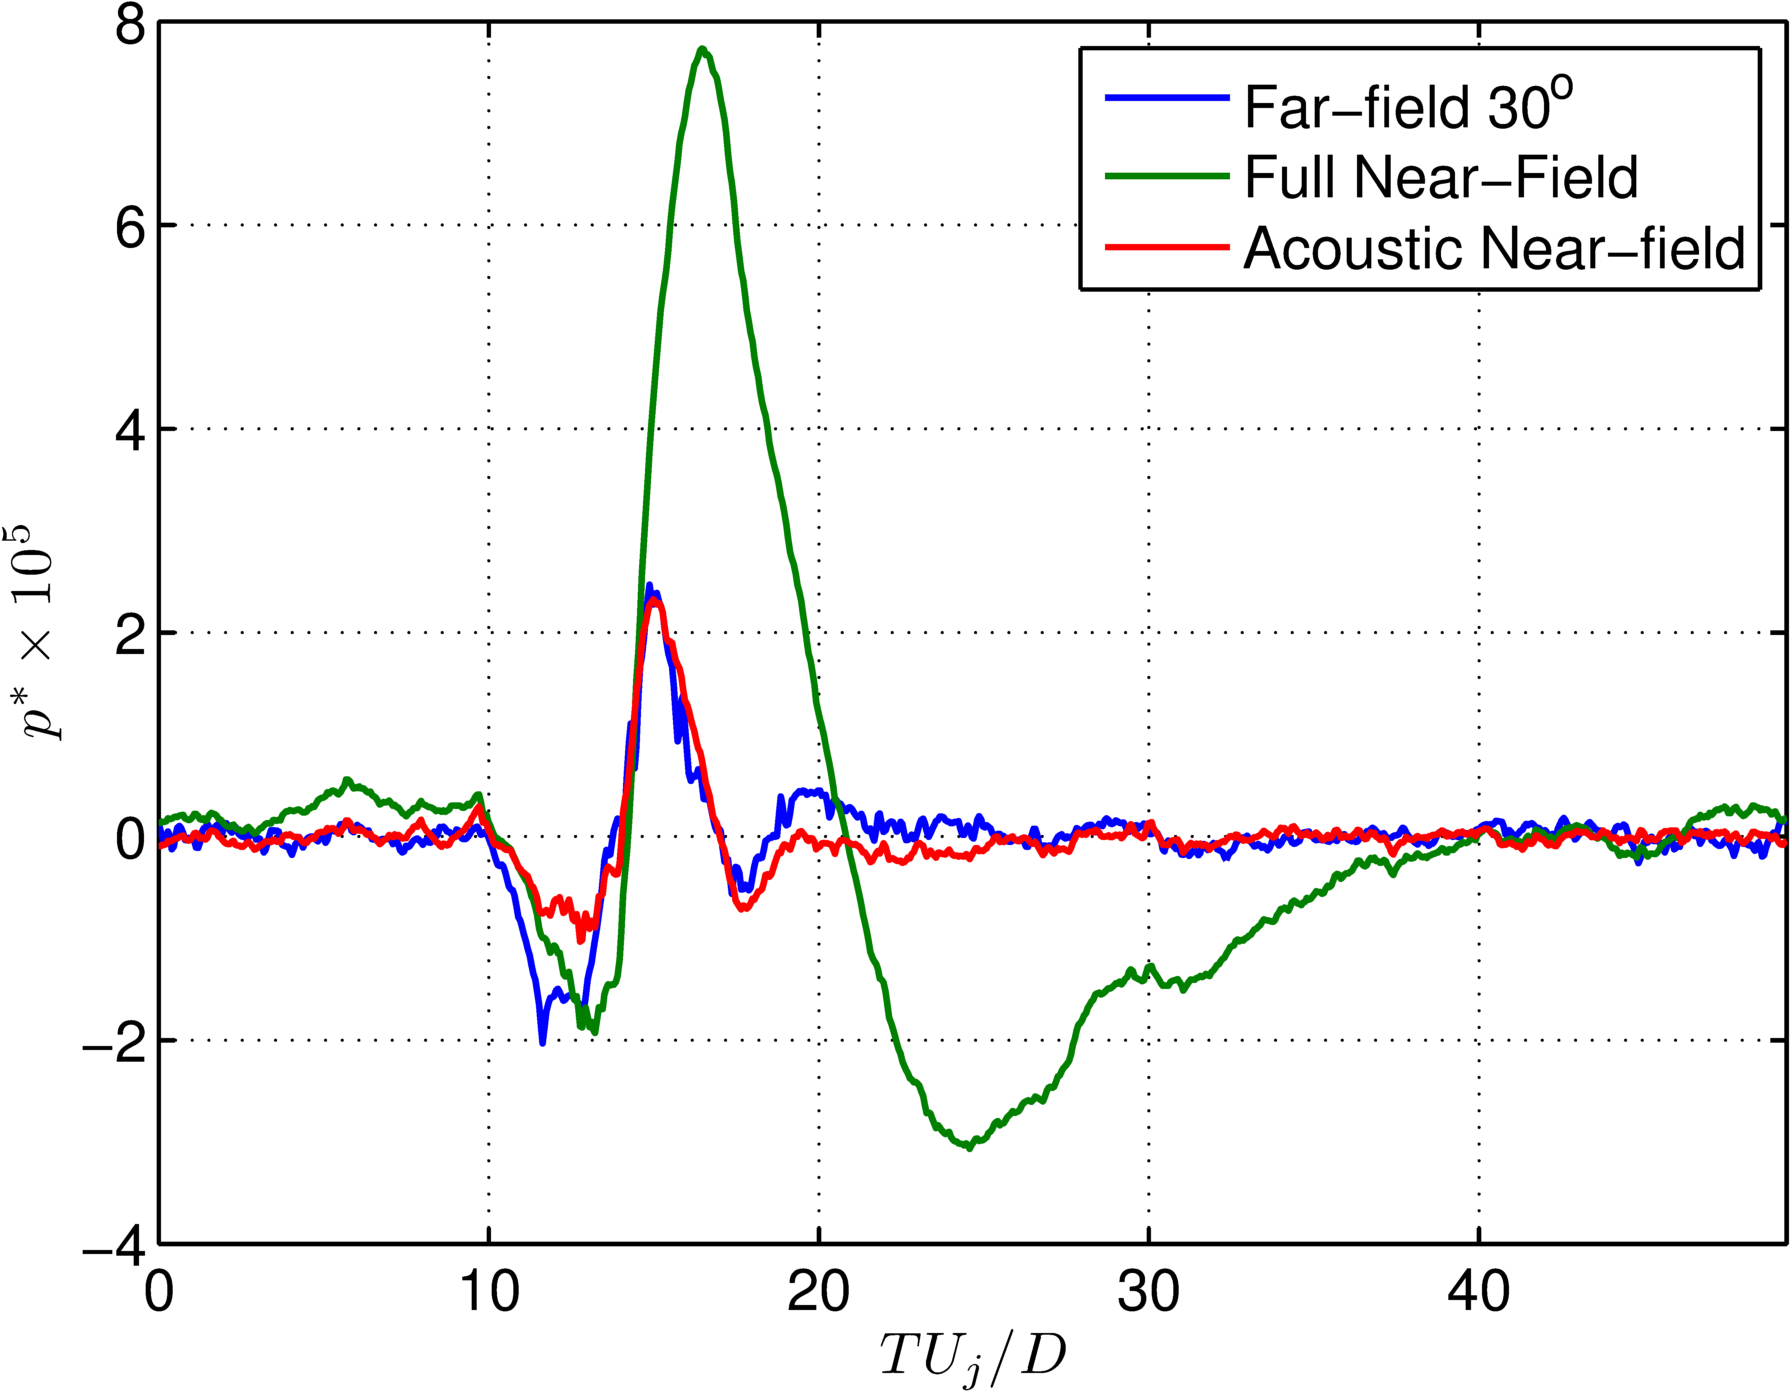
\includegraphics[width=3.25in]{EXP_DECOMP_NFvFF.png}}
	\caption{Comparison of full and decomposed near-field signal at $x/D = 8, y/D = 2.2$ propagated to the far-field at $30^o$, for the natural jet (a) and the jet excited at $St_{DF}= 0.02$ (b). }\label{EXP_DECOMP}
\end{figure}

A robust linkage directly between the hydrodynamic fluctuations and the noise emission is not a straightforward affair. 
However, initial associations can be made with two-point correlations between the near field and the far field. 
This was performed in the experimental jet for the closest array position to the far field at $30^{o}$ and the correlations were then examined in the spatio-temporal domain. 
Distinct regions of positive and negative correlation spanning several jet diameters and flow time scales are observed with drastically differing slopes, indicating differing propagation mechanisms. 
Similar to the work of Bogey \& Bailley\cite{bogey2007}, the physical phenomena to which these correlation regions correspond can be identified by comparing their slopes against the convective velocity of the large scale structures (indicated by $\tau_{con}$) and the ambient speed of sound (indicated by $\tau_{ac}$ for on-axis propagation between the near-field microphone and the far field and by $\tau_{s}$ for off-axis propagation). 
For simplicity, diffraction and convection effects have been neglected in this analysis. 
The convection velocity was assumed to be $U_{c} = 0.69U_{j}$; this value was determined from two-point correlations between adjacent microphones located in the most upstream region of the jet ($x/D \leq 5$).
The assumed source region, required to compute $\tau_{con}$ and $\tau_{s}$, is a free parameter that was set by the researchers subsequent to the computation of the two-point correlations in order to best match the observed correlation regions. 

Results from the natural jet in the experimental database can be found in Fig.~\ref{EXP_2ptcorr} for both the full near-field signal and the decomposed acoustic near field.
In the full near-field signal, four distinct correlation regions can be observed comprising two physical phenomena. 
In the most upstream region, the slopes of the correlations match the measured convective velocity of the large scale structures, with the peak correlation occurring just downstream of the end of the potential core ($x/D = 6$).
In order to align $\tau_{con}$ with the dominant convective correlation region, a source location of $x_{s}/D = 4$ was found to be necessary.
Beyond this location, these correlation regions merge with the second set of correlation regions, which exhibit a slope indicative of acoustically-propagating waves. 
These correlation regions start from almost negligible values upstream, strongly amplify near and just beyond the end of the potential core, and decay gradually in the downstream region.
The behavior of the acoustic correlation regions can, unsurprisingly, be better analyzed using the decomposed acoustic component of the near-field signal.
Here, no correlation regions matching the convective velocity of the large-scale structures exist; the convective correlation regions observed in Fig.~\ref{EXP_2ptcorr}a were associated with the large-scale structures themselves, rather than direct acoustic phenomena.
Instead, a single positive correlation region exists over the entire domain, roughly matching with $\tau_{ac}$.
A slight discrepancy is observed however in the furthest axial positions, where the positive correlation region instead matches with $\tau_{s}$, indicating a stationary source region. 
As before, a source location of $x_{s}/D = 4$ was found to produce the best match between $\tau_{s}$ and the observed correlation regions.
Similar behavior was observed for the excited jet, which for brevity is not included here. 
In the case of the excited jets, noticeably stronger convective correlations regions were observed, and a periodic pattern of oscillating positive and negative correlation regions, both in the convective and acoustic regions, was observed for the periodically excited jet.
Additionally, the source location was found to shift upstream with increasing excitation $St_{DF}$; this matches the upstream shift in the saturation point for higher $St_{DF}$ found in Fig.~\ref{pms}.
The behavior observed in these plots suggests that the dominant acoustic emissions (at least as identified by linear correlation) are being generated over an extended region of the jet, roughly $x/D \leq 4$, and that this location corresponds to the saturation point of the dominant large-scale structures.

\begin{figure}
	\centering{}\subfloat[]{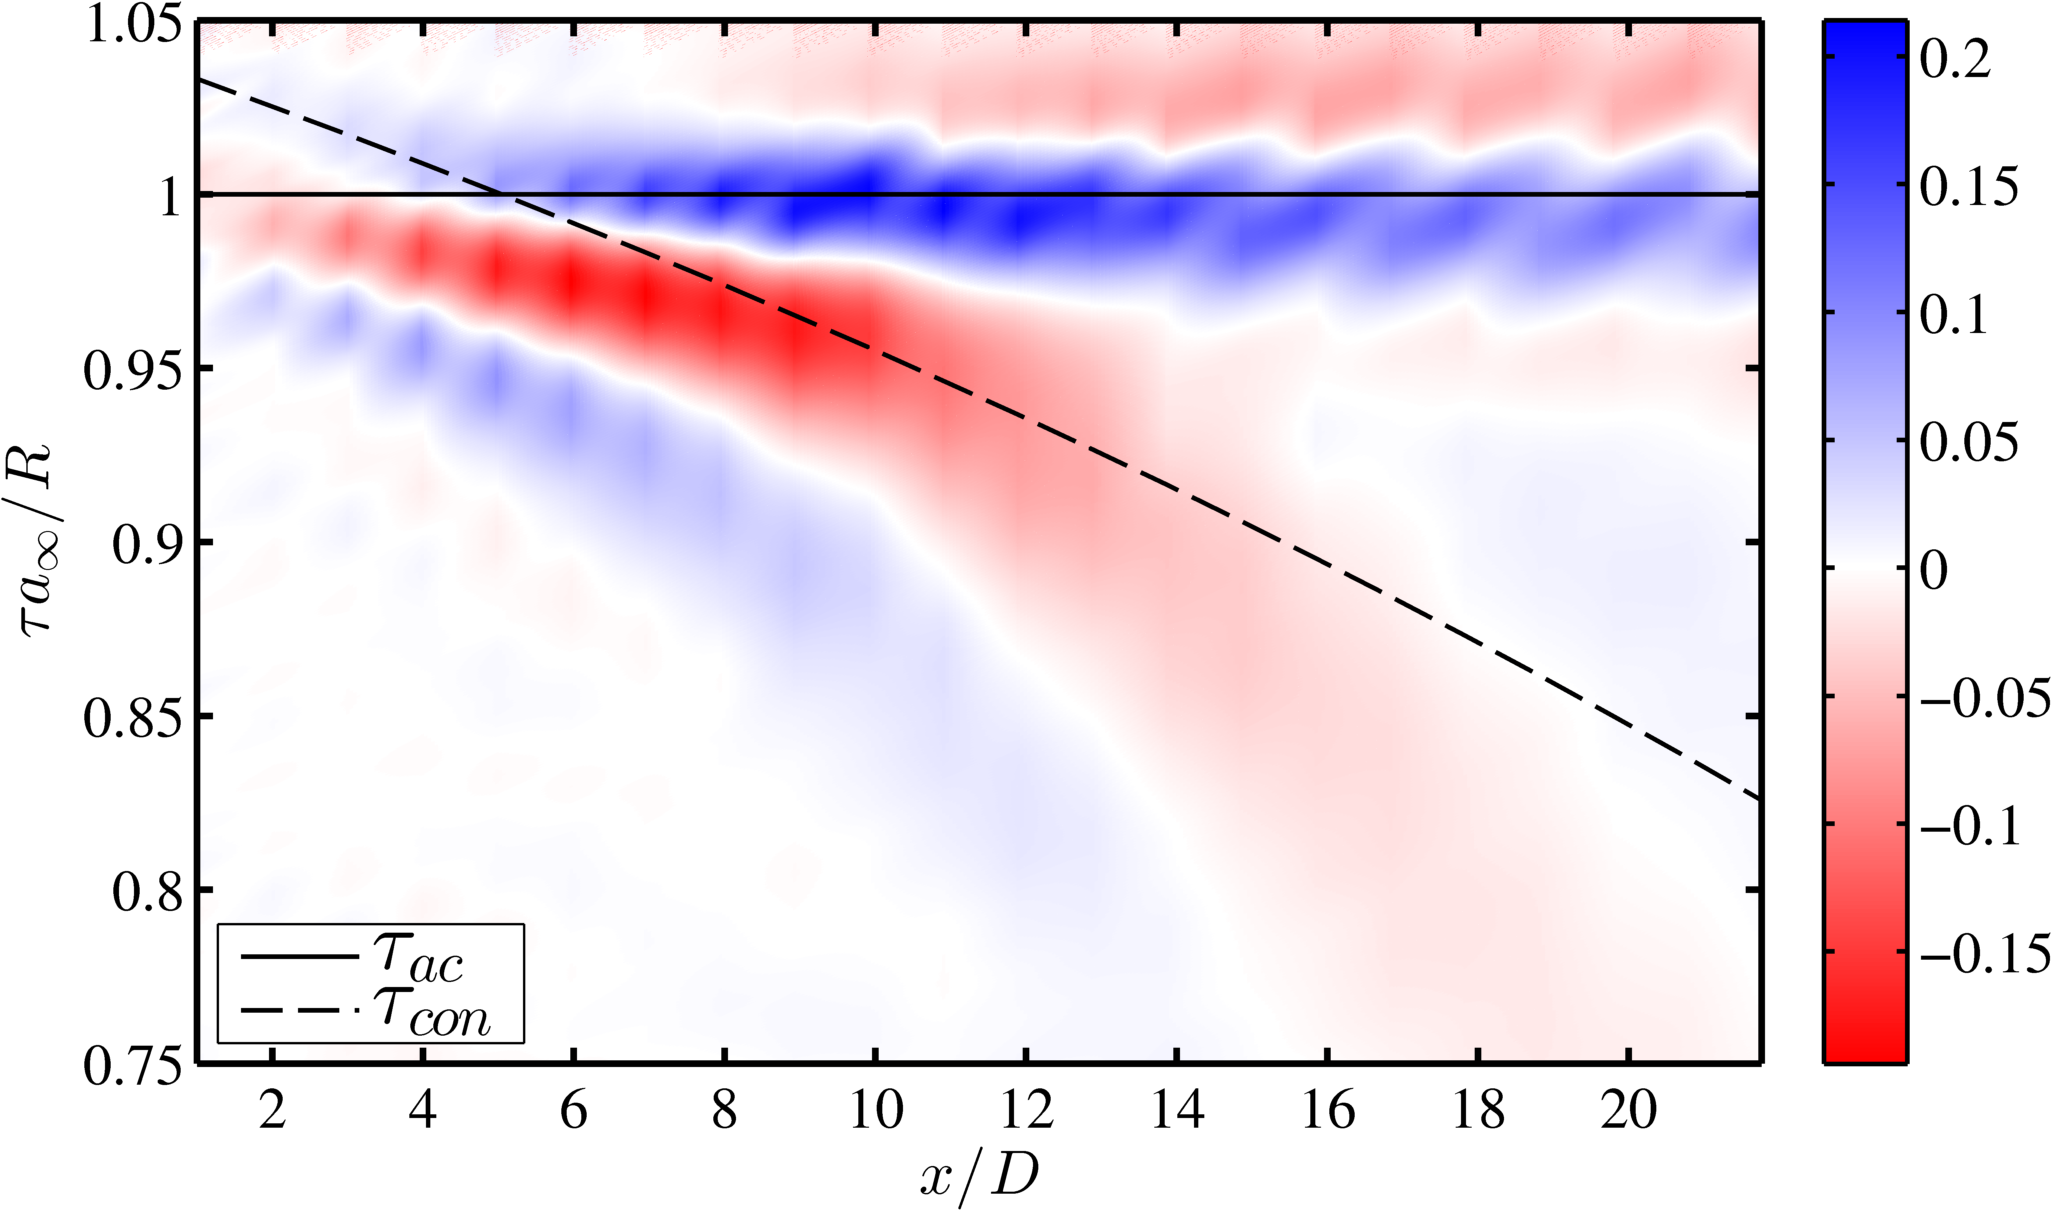
\includegraphics[width=3.25in]{St0_000_r1_20_ff30xcor_full.png}}\subfloat[]{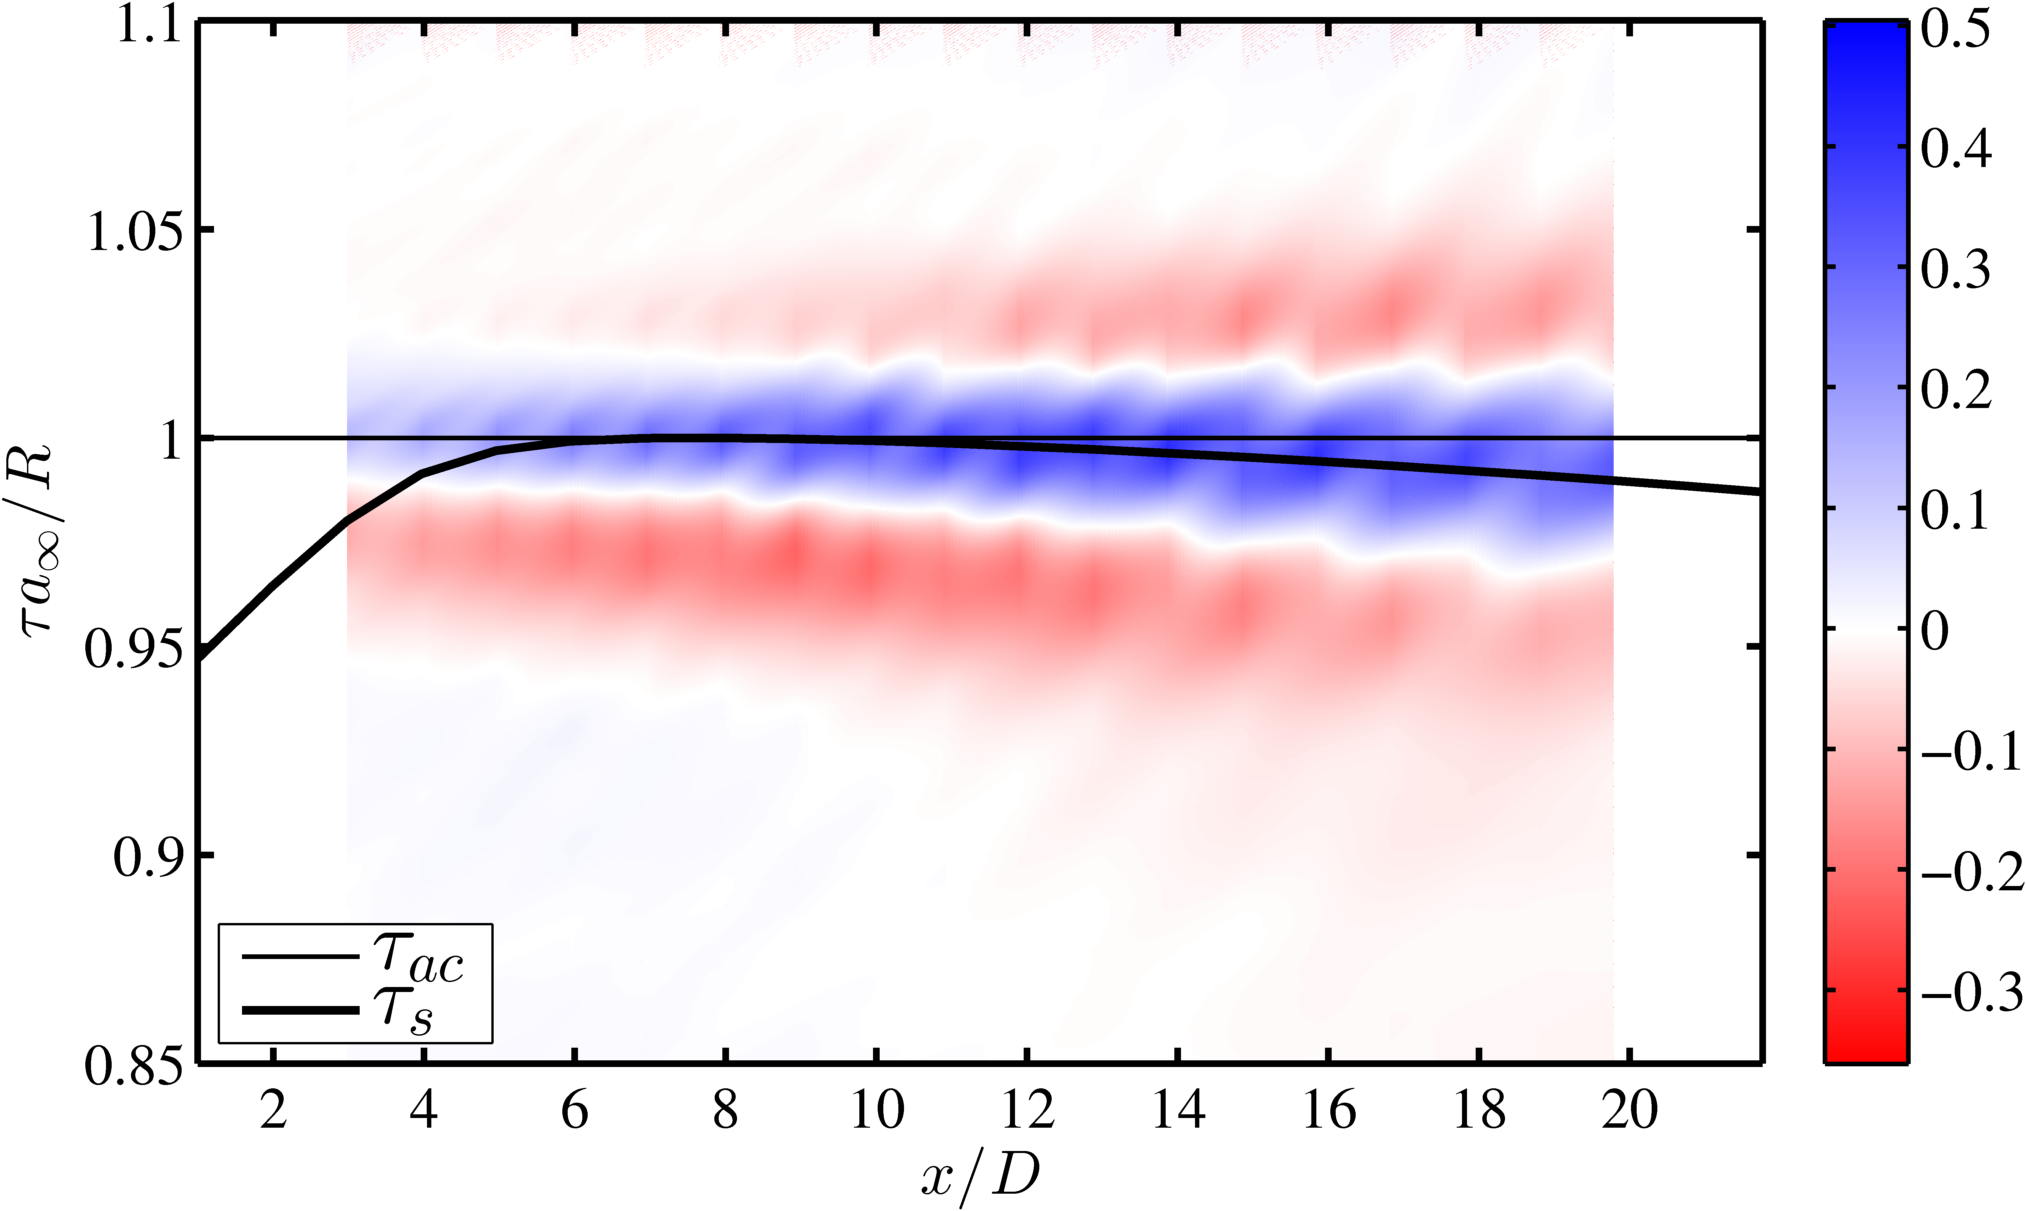
\includegraphics[width=3.25in]{St0_000_r1_20_ff30xcor_acoustic.png}}
	\caption{Two-point correlations between the full near-field (a) and acoustic component (b) in the experimental database to the far-field at $30^{o}$ for the natural jet. The near-field microphones were taken along the first array position, starting at $x/D = 1, y/D = 1.2$. The abscissa has been normalized by the ambient speed of sound and the distance from the near-field microphone to the far-field microphone.}\label{EXP_2ptcorr}
\end{figure}

As mentioned previously, the experimental database can only take the analysis so far, as we are unable to probe inside the mixing layer with both spatial and temporal high-fidelity with current experimental technology. 
Thus, analysis of the acoustic field embedded in the LES database is paramount. 
As a preliminary step, the phase-averaged waveforms generated by the excitation were again explored, this time at the furthest axial and radial position simulated (which corresponds to $x/D = 20.0, y/D = 9.0$ - due to computational limitations the acoustic far-field is not simulated).
Like the hydrodynamically-dominated waveforms shown in Fig.~\ref{NUM_Phase_AVG}, excitation of the jet at a very low $St_{DF}$ produces a compact, impulsive disturbance in the near acoustic field. 


\begin{figure}
	\centering{}{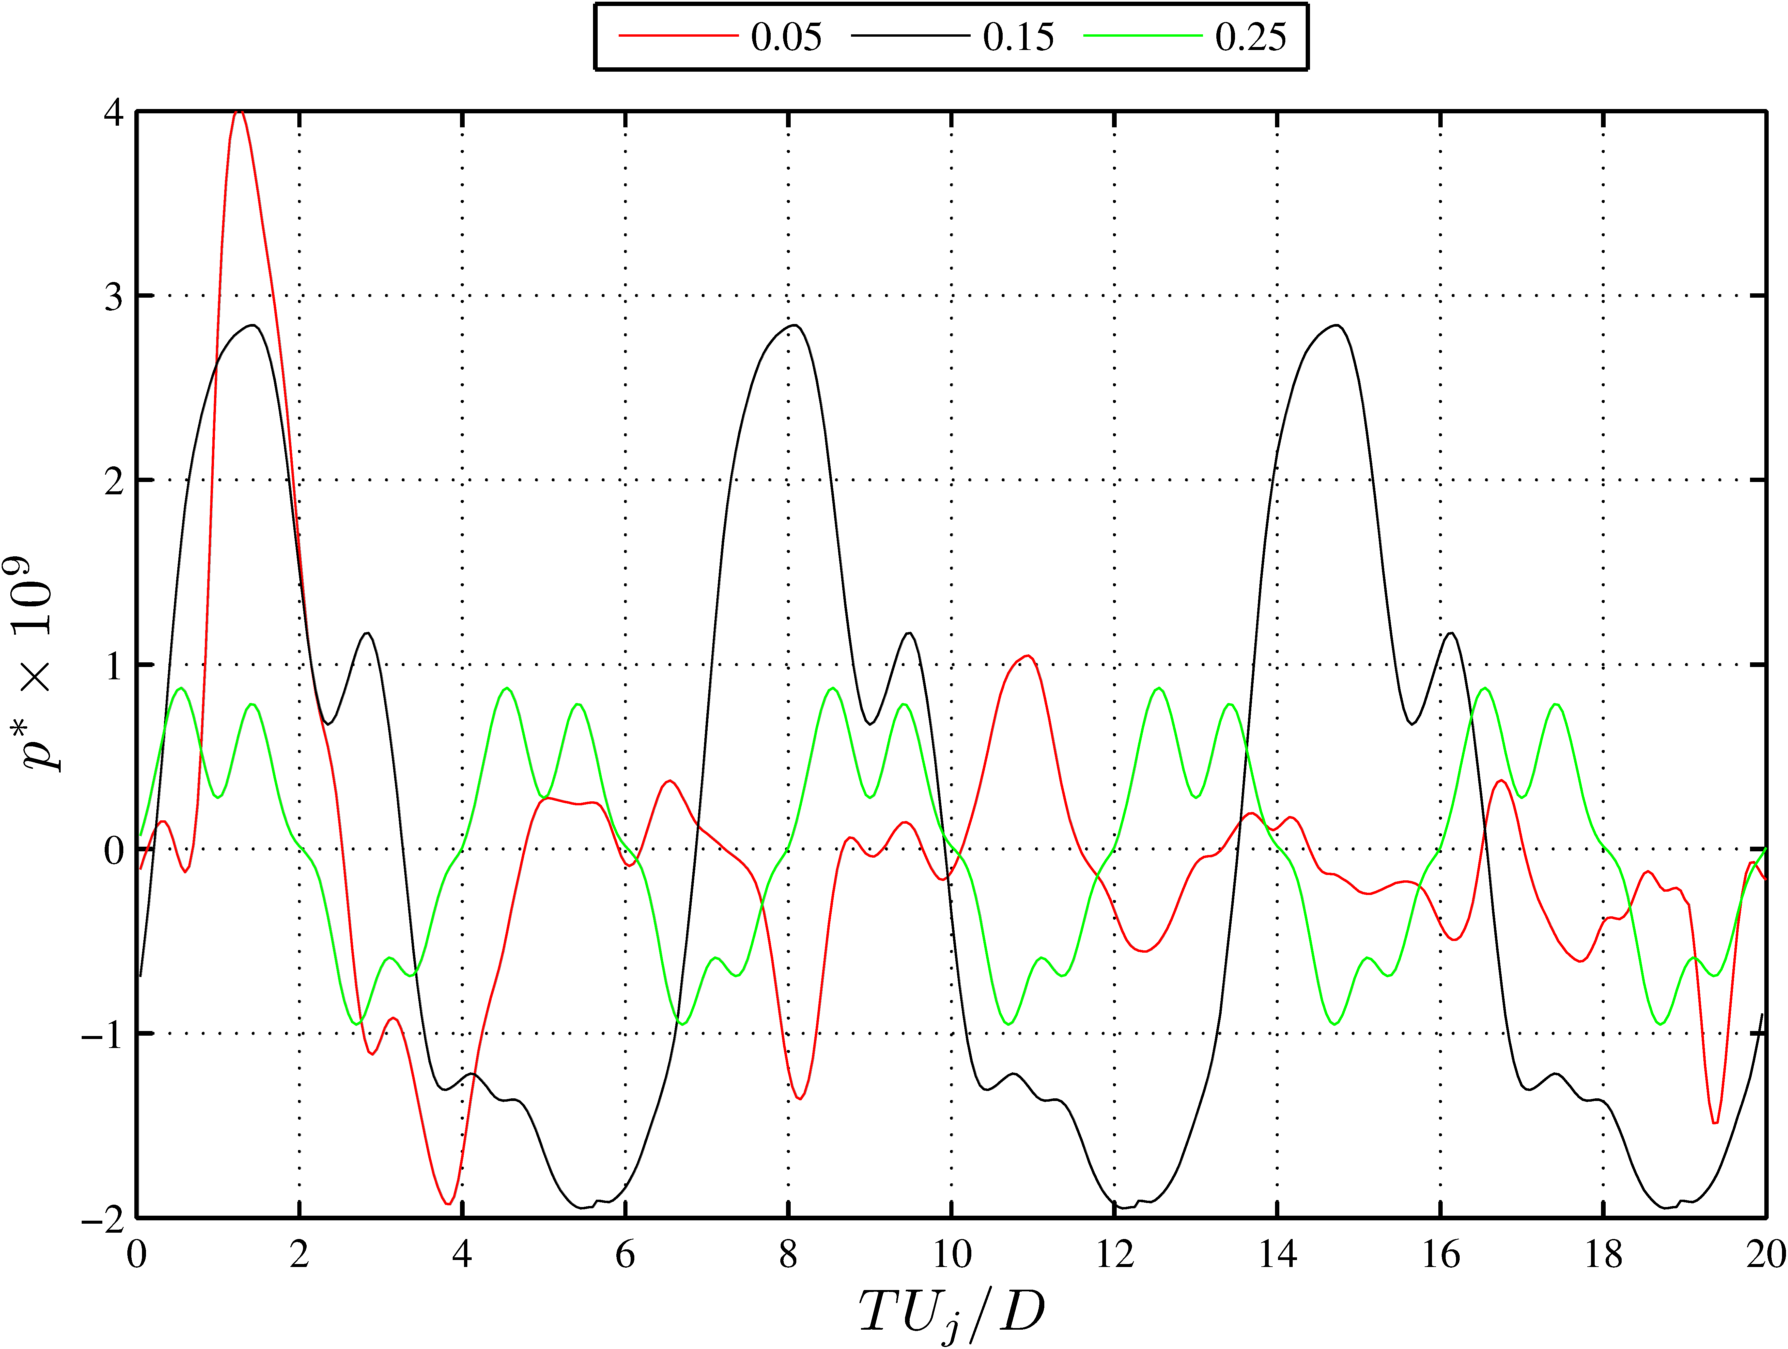
\includegraphics[width=3.25in]{Num_FFx1_phavg.png}}
	\caption{Response to excitation in the simulated jet, phase-averaged waveforms at $x/D = 20.0, y/D = 9.0$.}\label{NUM_FF}
\end{figure}

Similar to the experimental jet, two-point correlations between the full and decomposed near-field and the furthest axial and radial position were analyzed in order to located the dominant acoustic source region.
The full near-field was decomposed using the same methodology as that used for the experimental database. 
Hence, we are still restricted to decomposing the pressure field along an inclined array just outside the shear layer; as the decomposition occurs only in two dimensions, time and the axial direction, all fluctuations normal to the array appear to have a supersonic phase velocity.
If the array were to be located inside the shear layer, hydrodynamic fluctuations in the radial direction are misidentified as acoustic fluctuations. 
Therefore, the results shown in Fig.~\ref{Num_2ptcorr} used near-field locations which matched the first microphone array location in the experimental database (first microphone starts at $x/D = 1, y/D = 1.2$).
Work is currently underway in order to extend the wavelet filtering algorithm to higher spatial dimensions.
Even with the given restrictions, the acoustic source region quickly becomes apparent. 
As with the experimental results, the simulated database exhibits correlation regions which match quite well with the convective velocity of the large scale structures. 
Particularly in the case of the natural jet however, 
This does contrast with the behavior observed in the experimental jet, where the apparent source region in the natural jet does not differ significantly from the apparent source regions for the excited jets.

\begin{figure}
	\centering{}\subfloat[]{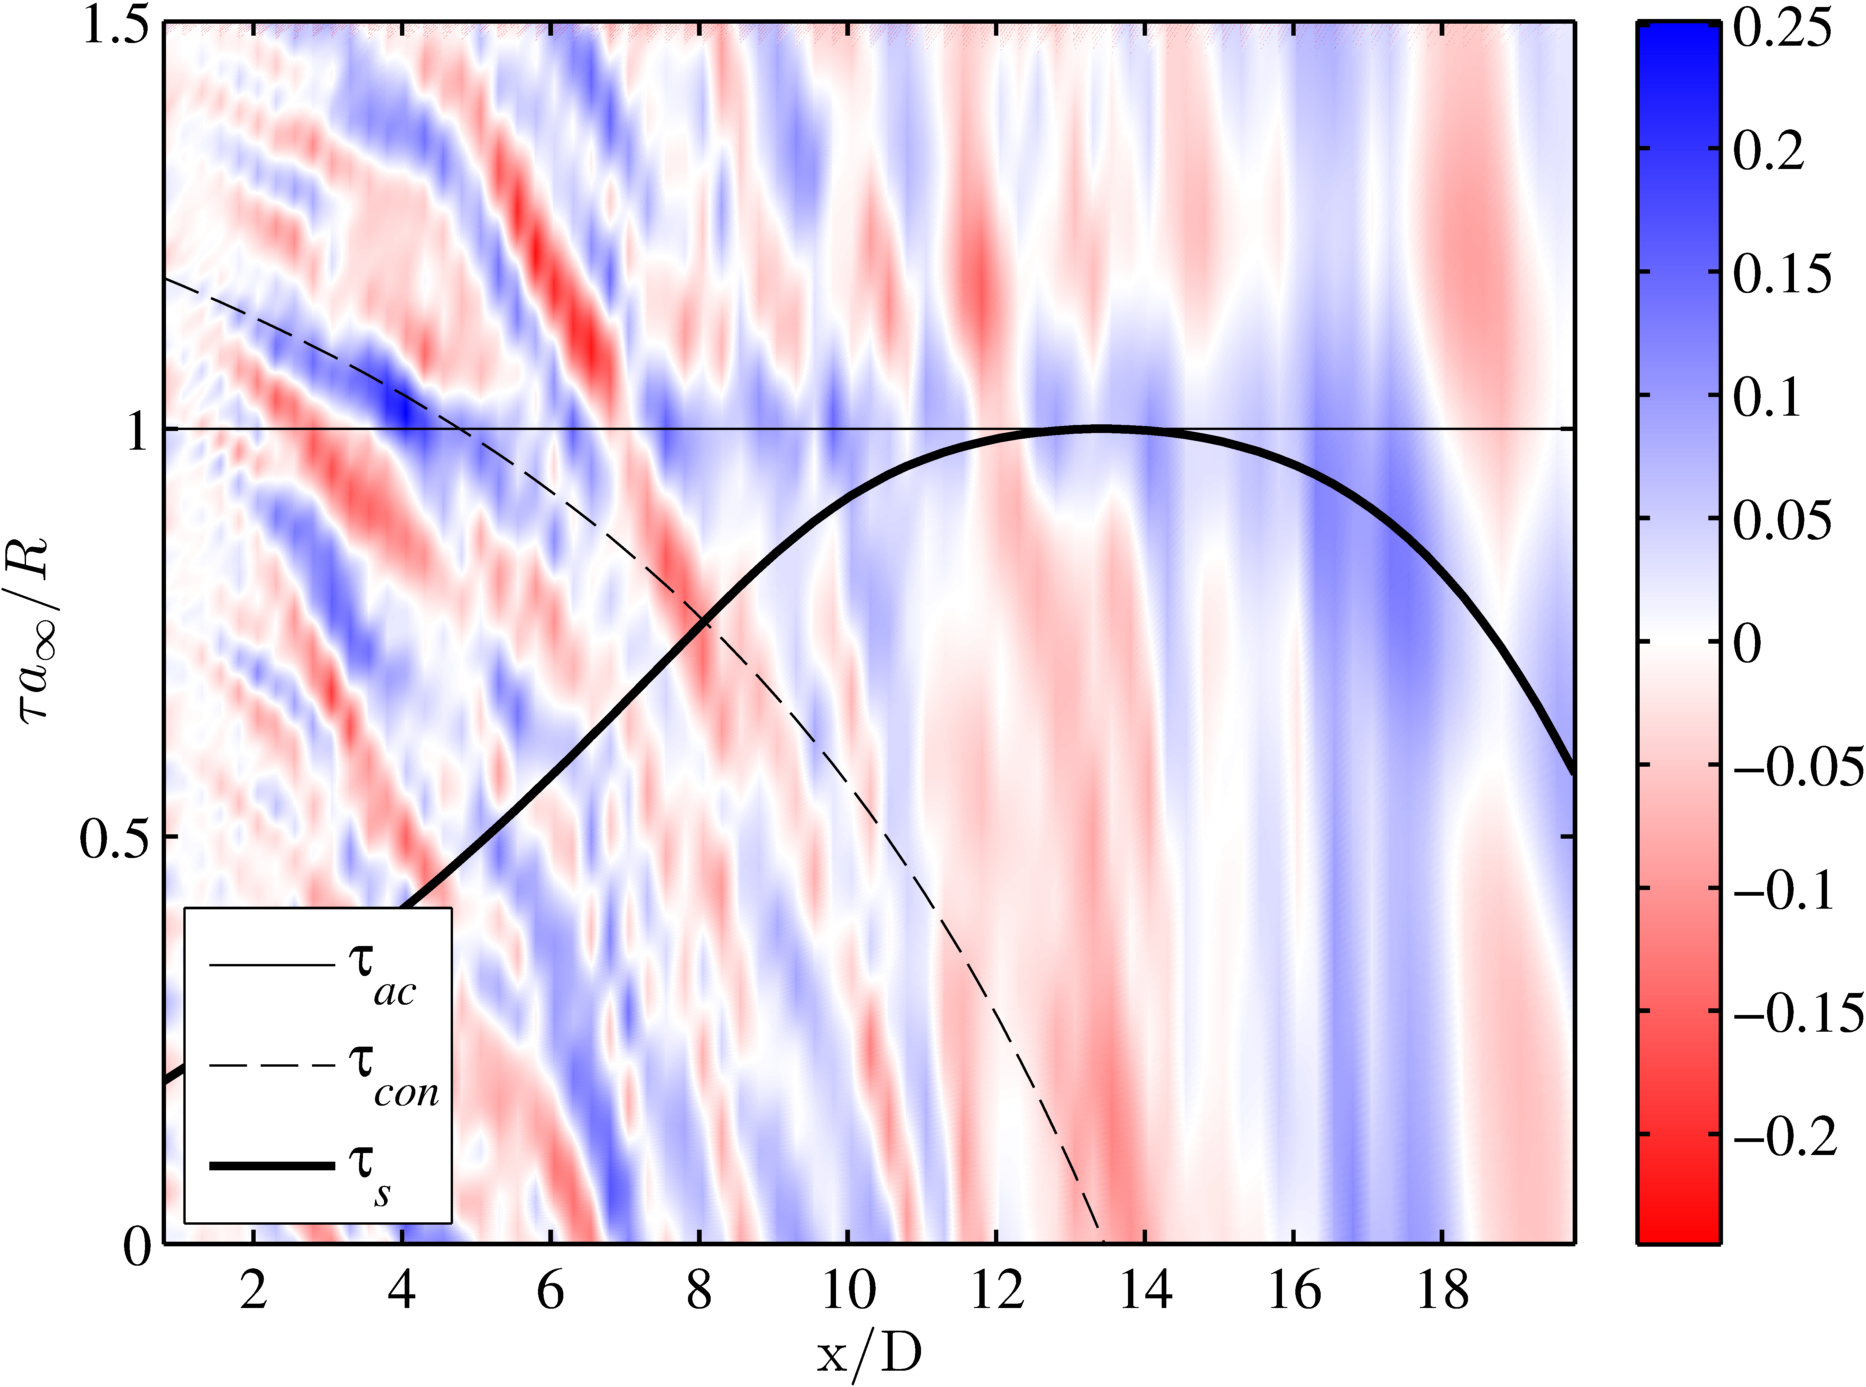
\includegraphics[width=3.25in]{Num_xcorr_NEARRAY1fullsignalsource10Dcorr.png}} \subfloat[]{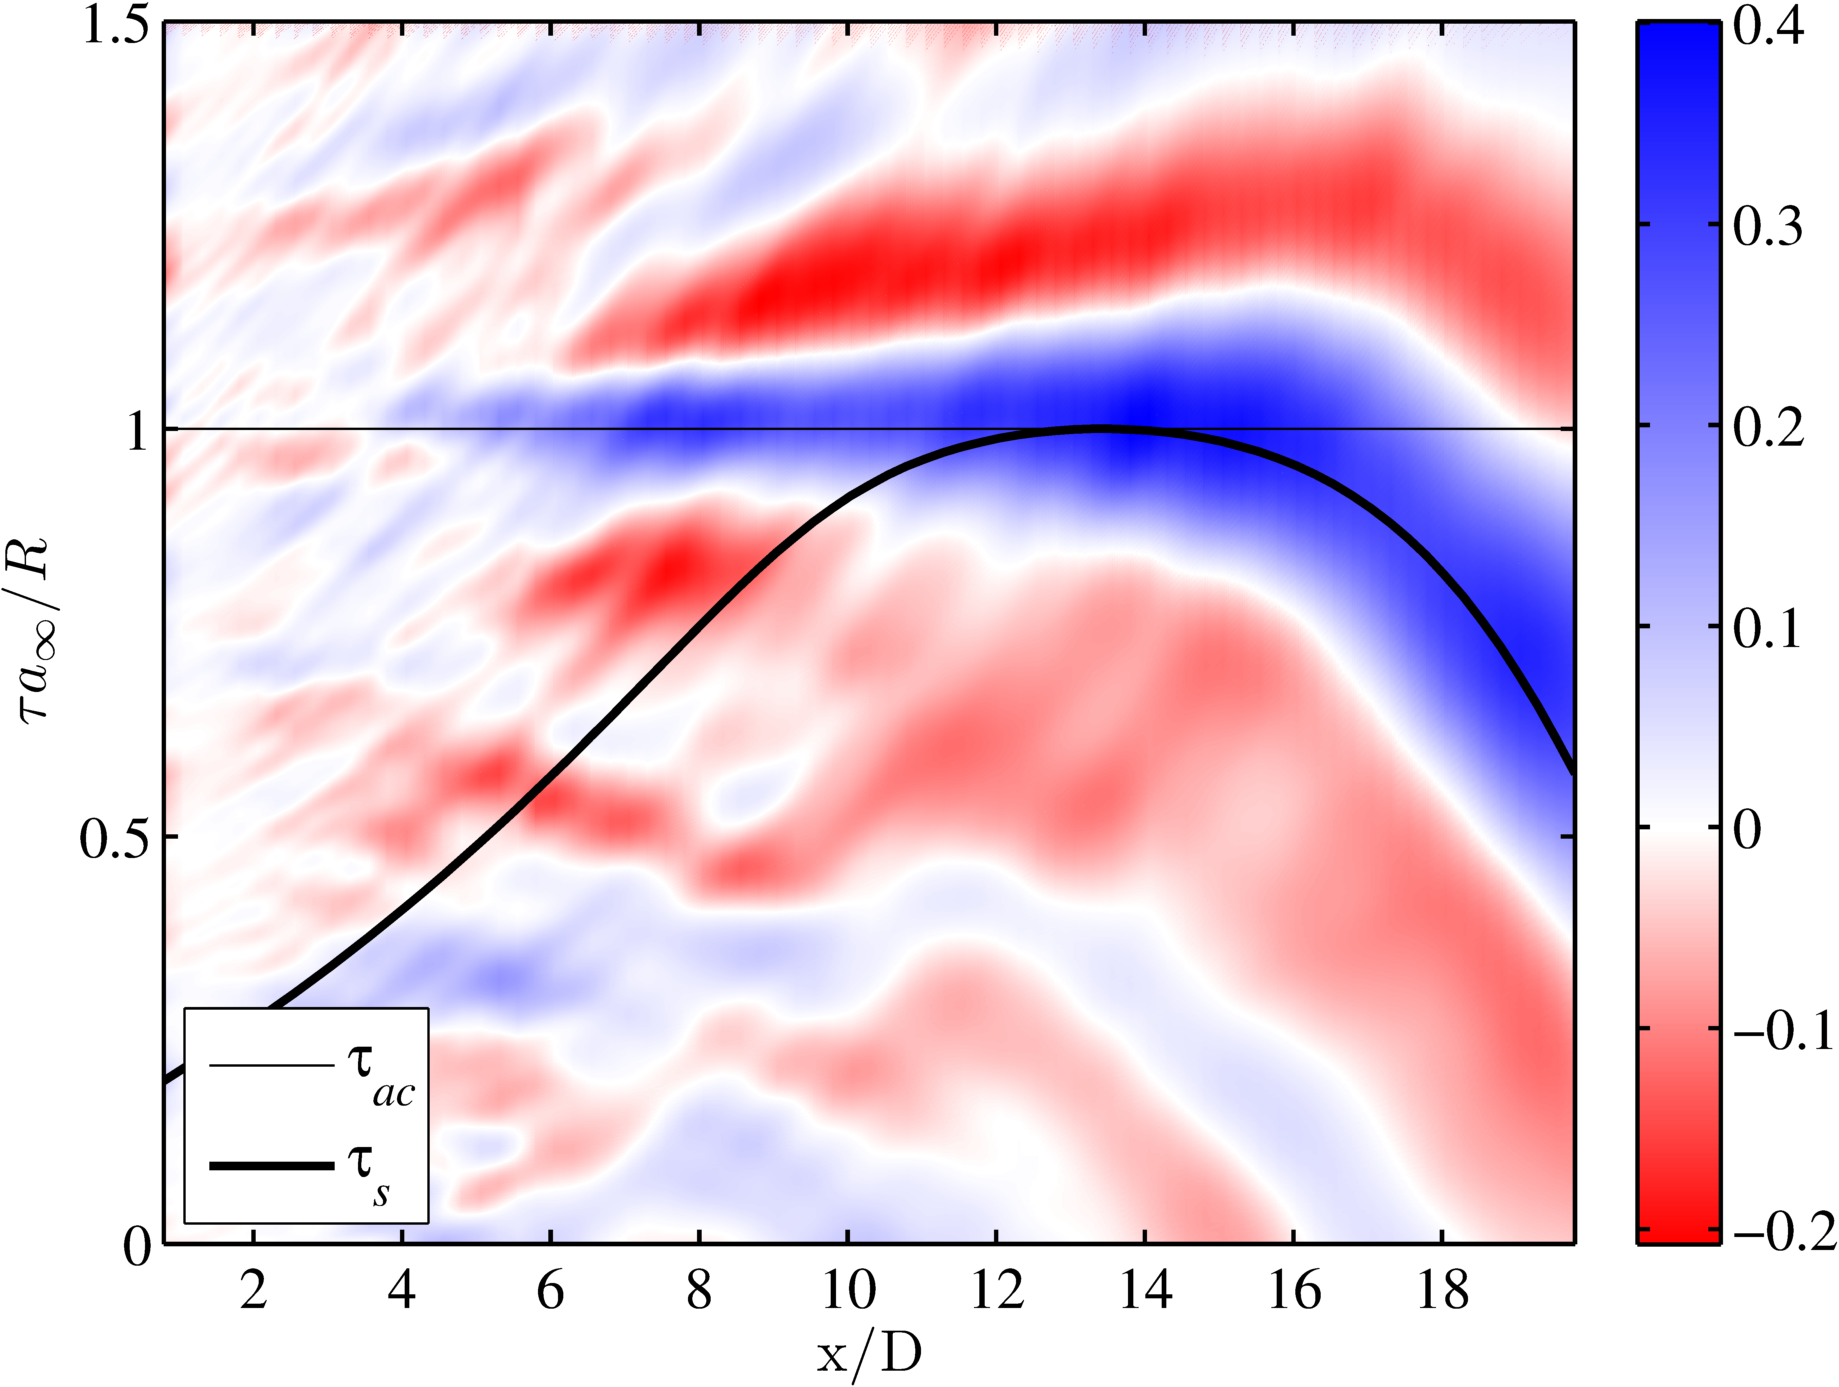
\includegraphics[width=3.25in]{Num_xcorr_NEARRAY1supsource10Dcorr.png}} 
	
	\subfloat[]{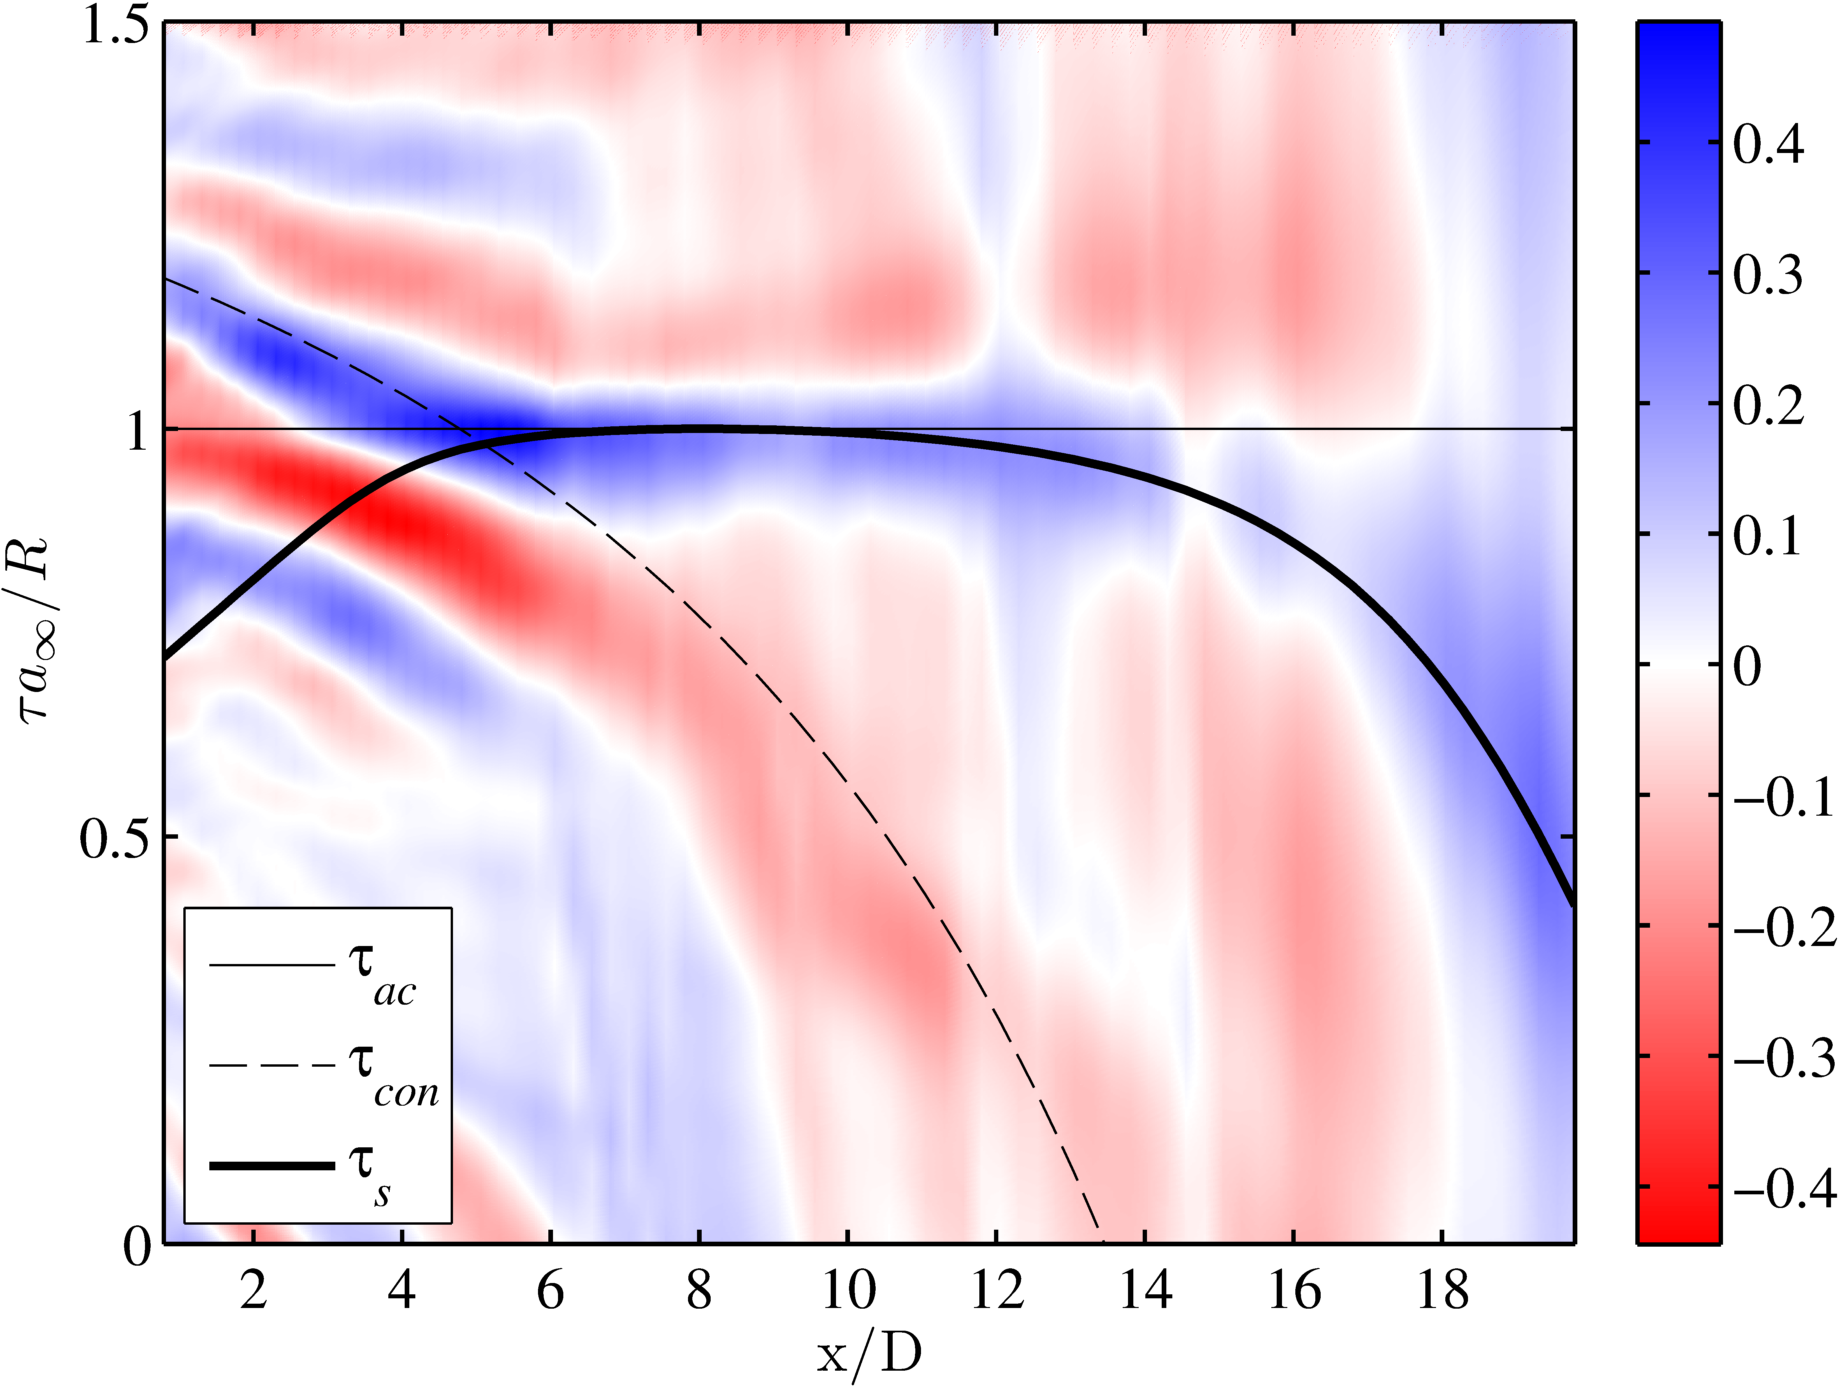
\includegraphics[width=3.25in]{Num_xcorr_fullsignalArray1St005.png}} \subfloat[]{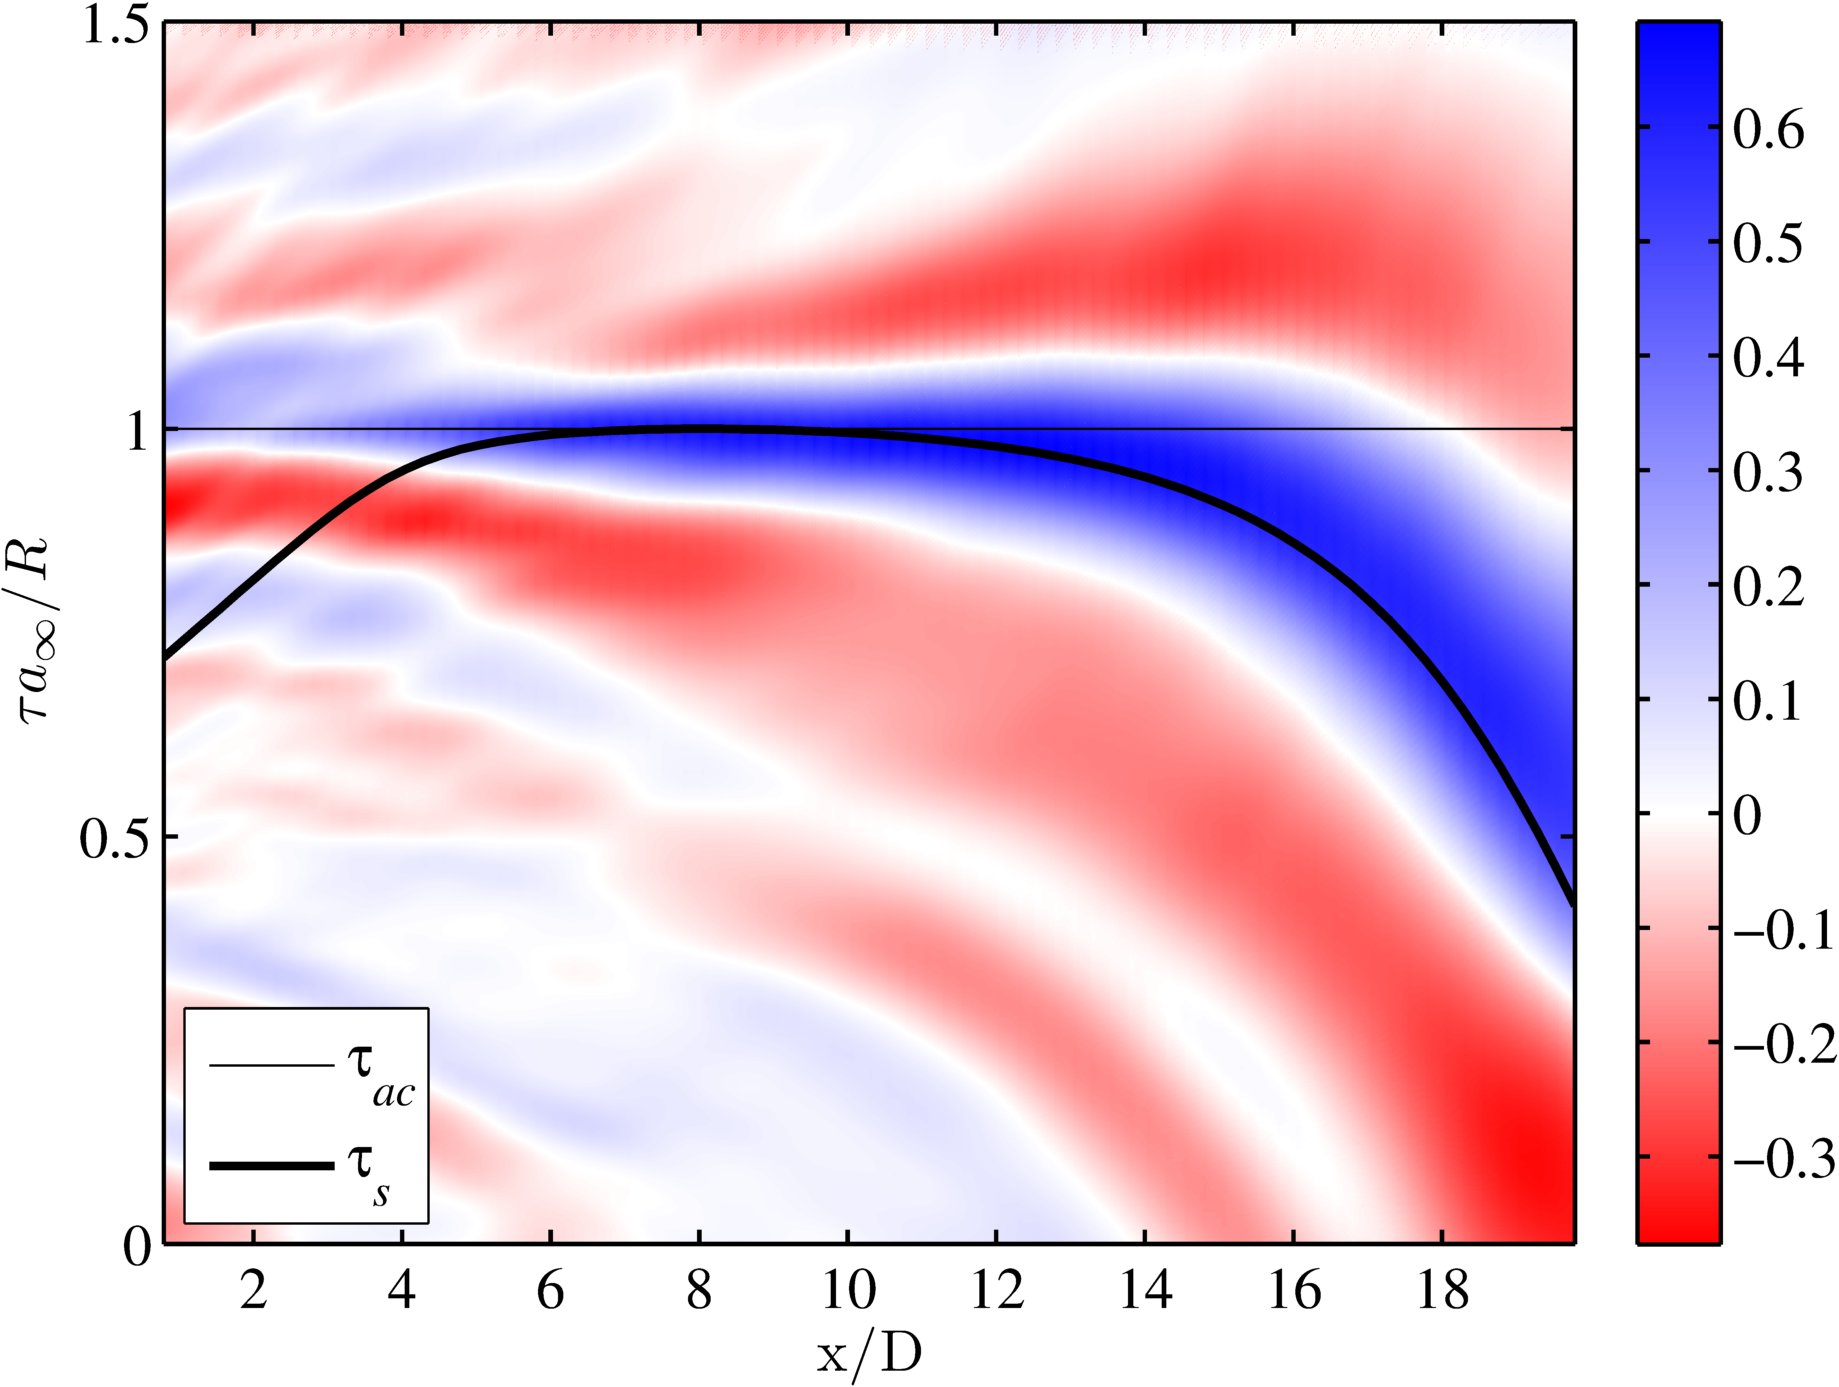
\includegraphics[width=3.25in]{Num_xcorr_St005superArray1corr.png}}
	\caption{Two-point correlations between the full near-field and acoustic component to the furthest downstream and radial position for the natural jet (a \& b, respectively) and the jet excited at $St_{DF} = 0.05$ (c \& d). Axial and radial positions match the location of the experimental array.}\label{Num_2ptcorr}
\end{figure}

\section{Conclusions and Future Work}
A Mach 0.9 jet was analyzed using results obtained from experiments and computations to understand the noise source mechanism and the resultant acoustic field. 
The linear superpositioning of phase-averaged waveforms shows that the large scale structures combine in a quasi-linear fashion for both the experiments and the computations. 
Two-point correlations were used to compare the near jet (hydrodynamically dominant) region to the acoustically dominant near and far fields. 
The full signal of the near field was also decomposed into hydrodynamic and acoustic portions through a wavelet decomposition technique. 
These signals were correlated to the acoustic field to characterize the dependence of specific regions of the jet to the far field sound.

\section*{Acknowledgments}
   Computational resources were provided by the DoD HPCMP (AFRL, NAVO
   and ERDC) and the Ohio Supercomputer Center. The support of this
   complementary experimental and computational work by the Air Force
   Office of Scientific Research (Dr. John Schmisseur and
   Dr. Rengasamy Ponnappan) is greatly appreciated. Several figures
   were made using Fieldview software with licenses obtained from the
   Intelligent Light University Partnership Program. 

\bibliographystyle{aiaa}
\bibliography{./NEWMASTER}
%\printnomenclature

\end{document}
